\documentclass[12pt, a4paper, oneside]{ctexart}
\usepackage{amsmath, amsthm, amssymb, bm, color, graphicx, geometry, mathrsfs,extarrows, braket, booktabs, array, listings, xcolor, fontspec, appendix, float, subfigure, wrapfig}
\usepackage[colorlinks,linkcolor=red,anchorcolor=blue,citecolor=blue,urlcolor=blue,menucolor=black]{hyperref}

%%%%%% 设置代码块 %%%%%%
\usepackage{minted}
\renewcommand{\theFancyVerbLine}{
    \sffamily\textcolor[rgb]{0.5,0.5,0.5}{\scriptsize\arabic{FancyVerbLine}}} % 修改代码前序号大小
\setmainfont{Times New Roman}  % 设置英文字体
\setsansfont{Calibri}
\setmonofont{Consolas}
\newmintinline{python}{linenos, breaklines, frame=lines, python3}  % 使用\pythoninline{代码}
\newminted{python}{linenos, breaklines, frame=lines, python3}  % 使用\begin{pythoncode}代码\end{pythoncode}
\newmintedfile{python}{linenos, breaklines, frame=lines, python3}  % 使用\pythonfile{代码地址}

%%%%%% 设置字号 %%%%%%
\newcommand{\chuhao}{\fontsize{42pt}{\baselineskip}\selectfont}
\newcommand{\xiaochuhao}{\fontsize{36pt}{\baselineskip}\selectfont}
\newcommand{\yihao}{\fontsize{28pt}{\baselineskip}\selectfont}
\newcommand{\erhao}{\fontsize{21pt}{\baselineskip}\selectfont}
\newcommand{\xiaoerhao}{\fontsize{18pt}{\baselineskip}\selectfont}
\newcommand{\sanhao}{\fontsize{15.75pt}{\baselineskip}\selectfont}
\newcommand{\sihao}{\fontsize{14pt}{\baselineskip}\selectfont}
\newcommand{\xiaosihao}{\fontsize{12pt}{\baselineskip}\selectfont}
\newcommand{\wuhao}{\fontsize{10.5pt}{\baselineskip}\selectfont}
\newcommand{\xiaowuhao}{\fontsize{9pt}{\baselineskip}\selectfont}
\newcommand{\liuhao}{\fontsize{7.875pt}{\baselineskip}\selectfont}
\newcommand{\qihao}{\fontsize{5.25pt}{\baselineskip}\selectfont}

%%%% 下面的命令设置行间距与页边距 %%%%
\linespread{1.2}
\geometry{left=2.5cm, right=2.5cm, top=2.5cm, bottom=2.5cm}

%%%% 正文开始 %%%%
\begin{document}

%%%% 定理类环境的定义 %%%%
\newtheorem{example}{例}             % 整体编号
\newtheorem{theorem}{定理}[section]  % 按 section 编号
\newtheorem{definition}{定义}
\newtheorem{axiom}{公理}
\newtheorem{property}{性质}
\newtheorem{proposition}{命题}
\newtheorem{lemma}{引理}
\newtheorem{corollary}{推论}
\newtheorem{remark}{注解}
\newtheorem{condition}{条件}
\newtheorem{conclusion}{结论}
\newtheorem{assumption}{假设}
\numberwithin{equation}{section}  % 按章节编号
\newtheorem{algorithm}{算法}

%%%% 重定义 %%%%
\renewcommand{\contentsname}{目录}  % 将Contents改为目录
\renewcommand{\abstractname}{摘要}  % 将Abstract改为摘要
\renewcommand{\refname}{参考文献}   % 将References改为参考文献
\renewcommand{\indexname}{索引}
\renewcommand{\figurename}{图}
\renewcommand{\tablename}{表}
\renewcommand{\appendixname}{附录}
%\renewcommand{\algorithm}{算法}
\graphicspath{{figure/}}  % 图片相对路径

% 一些宏定义
\def\bd{\boldsymbol}
\def\disp{\displaystyle}
\def\sign{\text{sign}}
\def\wtd{\widetilde}
\def\bR{\mathbb{R}}
\def\wdh{\widehat}
\def\L{\mathcal{L}}
\def\add{\vspace{1ex}}  % 增加行间距
\def\del{\vspace{-3.5ex}}  % 减少行间距


%%%% 定义标题格式,包括title,author,affiliation,email等 %%%%
\title{最优化方法\\多层神经网络的训练问题}
\author{
西安交通大学, 数学与统计学院, 强基数学002\\[3ex]
吴天阳$^a$, 马煜璇$^b$, 白鹏楠$^c$\\[1ex]
2204210460$^a$, 2204220461$^b$, 2204421343$^c$\\[2ex]
}
\date{2022年4月18日}

\maketitle % 设置上面是标题
\clearpage
\tableofcontents % 创建目录,使用目录需要编译两次,并且不能删去编译产生的临时文件!!!

%%%% 以下部分是正文 %%%%  
\clearpage

\section{神经网络介绍}
随着神经科学、认知科学的发展, 我们逐渐发现人类的智能行为和大脑的活动有关, 人类的大脑是一个能够产生意识、思想和情感的复杂器官. 受到人类大脑大脑的启发, 早期的神经科学家构造了一种模仿人脑神经系统的数学模型, 称为\textbf{人工神经网络}(Artificial Neural Network), 简称神经网络. 在机器学习领域, 神经网络是指由很多\textbf{人工神经元}构成的网络结构, 每个人工神经元之间的连接强度是\text{可学习参数}. 

\begin{wrapfigure}[13]{r}{.5\linewidth}
    \centering
    \label{figure-神经网络}
    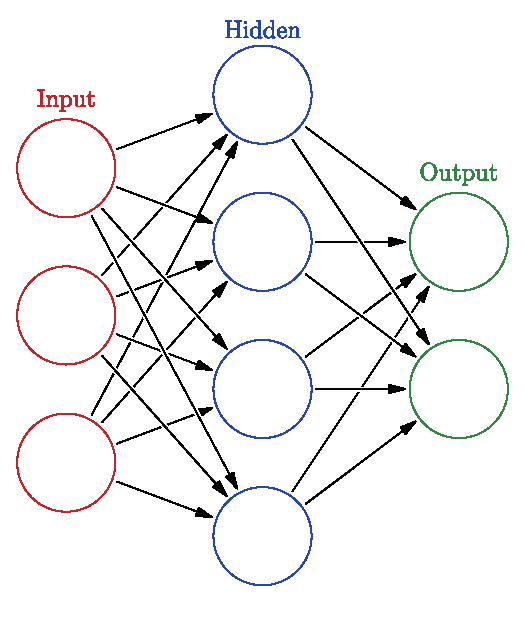
\includegraphics[scale=0.7]{neural_network.eps}
    \caption{神经网络结构\protect\footnotemark[1]}
\end{wrapfigure}
\footnotetext[1]{图片来源: \url{https://en.wikipedia.org/wiki/File:Colored_neural_network.svg}}

如图\ref{figure-神经网络}是一个人工神经网络, 它由三层组成, 分别为\textbf{输入层、隐藏层、输出层}. 每一个圆圈结点代表一个人工神经元, 每一个箭头代表神经元之间从输入到输出方向的连接, 并包含一个权重值, 表示两个神经元之间的连接强度. 每一个各人工神经元可以视为一种有多个参数确定的函数, 先将来自前一层节点的信息经过相应的权重综合计算, 再输入到一个激活函数中, 从而获得当前节点的活性值.

\subsection{模型}

从数学的角度来看神经网络, 其本质就是一种由大量参数确定的复杂的非线性函数. 对于一个机器学习任务, 我们可以认为是给出一些样本, 每个\textbf{样本}由输入向量$\bd{x}$和其对应的输出值$y$所决定, 记为$(\bd{x}, y)$, 所有样本构成一个\textbf{样本空间}$\mathcal{X}\times \mathcal{Y}$, 即对于任意一个样本都有$(\bd{x},y)\in \mathcal{X}\times\mathcal{Y}$, 假定存在一个未知的\textbf{真实映射函数}$g:\mathcal{X}\rightarrow \mathcal{Y}$, 使得对于每一个样本$(\bd{x}, y)$都有$g(\bd{x}) = y$, 机器学习的目标就是去近似真实映射函数$g(\bd{x})$.

由于不知道真实映射函数$g(\bd{x})$的具体形式, 于是只能假设一个函数集合$\mathcal{F}$, 称为\textbf{假设空间}(Hypothesis Space), 通过大量样本对网络的训练, 从中选取一个理想的\textbf{假设}(Hypothesis) $f^*\in \mathcal{F}$. 假设空间一般是一个参数化的函数族
\begin{equation}
    \mathcal{F} = \{f(\bd{x}; \theta):\theta\in \bR^D\},
\end{equation}
其中$f(\bd{x};\theta)$是参数为$\theta$的函数, 也称为\textbf{模型}(Model), $D$为参数的数量.

\subsubsection{线性模型}
线性模型的假设空间为一个参数化的线性函数族, 即
\begin{equation}
    f(\bd{x};\theta) = f(\bd{x}:\bd{w}, b) = \bd{w}^T\bd{x}+b,
\end{equation}
其中参数$\theta$包含权重向量$\bd{w}$和偏置$b$, 下文中的\hyperref[section-感知器算法]{感知器算法}就是一种线性模型.

\subsubsection{非线性模型}
广义的非线性模型可以写成多个非线性\textbf{基函数}$\phi(\bd{x})$的线性组合
\begin{equation}
    f(\bd{x};\theta) = \bd{w}^T\phi(\bd{x})+b,
\end{equation}
其中$\phi(\bd{x}) = [\phi_1(\bd{x}),\phi_2(\bd{x}),\cdots,\phi_K(\bd{x})]^T$为$K$个非线性基函数组成的向量, 参数$\theta$包含了权重向量$\bd{w}$和偏置$b$.

如果$\phi(\bd{x})$本身也为可学习基函数, 即
\begin{equation}\label{eq-基函数}
    \phi_k(\bd{x}) = h(\bd{w}_k^T\phi'(x)+b_k),\quad k=1,2,\cdots, K,
\end{equation}
其中$h(\cdot)$为非线性函数, $\phi'(\bd{x})$为另一组基函数, $\bd{w}_k$和$b_k$可学习参数, 则$f(\bd{x}; \theta)$就等价于\textbf{神经网络模型}. 

如果我们将第$s$层中从上至下第$k$个人工神经元视为函数$\phi_k^{(s)}(\bd{x})$, 那么一层中所有神经元构成函数向量$\phi^{(s)}(\bd{x})$, 由于当前层的神经元$\phi^{(s)}(\bd{x})$是由上一层的所有神经元$\phi^{(s-1)}(\bd{x})$通过权重矩阵$\bd{w}^{(s)}$计算加上偏置$b^{(s)}$, 再经过一个非线性激活函数$h(\cdot)$得到的, 即$\phi^{(s)}(\bd{x}) = h(\bd{w}^{(s)T}\phi^{(s-1)}(\bd{x})+b^{(1)})$满足式(\ref{eq-基函数}), 所以可以看出神经网络的本质就是从输入空间到输出空间的非线性参数化函数.

\subsection{神经网络的类型}

\hyperref[section-感知器算法]{感知器}是最早具有机器学习思想的神经网络, 也是最简单的人工神经网络, 我们将从感知器算法为例, 阐述机器学习的基本概念和符号定义. 神经网络模型分为主要的三种, 分别为\textbf{前馈型神经网络、卷积神经网络和循环神经网络}, 还有一种更一般性的网络: \textbf{图网络}, 由于时间所限, 我们只研究了前馈型神经网络模型的理论基础及实际应用.

\section{感知器算法}\label{section-感知器算法}
\textbf{感知器(Perceptron)}是Frank Rosenblatt于1957年所发明的, 它可以被视为一种最简单的前馈神经网络.

感知器是一种\textbf{二元线性分类器(Binary Linear Classifier)}, 大概地来说, 感知器的输入为样本的\textbf{特征向量}, 输出为样本的类别, 以$+1$表示正类, $-1$表示负类, 利用\textbf{随机梯度下降法}对\textbf{损失函数}进行极小化, 求出可将样本进行划分的\textbf{分离超平面}.
\subsection{感知器模型}
我们通过一个例子引入: 预测学生能否通过课程的问题, 对于一名学生, 根据一批与这门课程相关的数据, 预测他是否可以通过某一门课程. 与这门课程相关的每一种数据称为\textbf{特征(Feature)}, 我们用$n$维向量$\bd{x}$进行存储, $\bd{x}$中的每一维对应一种特征, 称$\bd{x}$为\textbf{特征向量(Feature Vector)}. 比如:第一个维度$x_1$为出勤率, 第二个维度$x_2$为自主学习时长等等.我们将这些维度的数据加权求和, 得到一个综合得分$\sum_{i=1}^nw_ix_i$, 如果该得分高于某个标准$b$, 则预测他可以通过, 否则不能通过.现在假设我们有大量该课程的历史学生数据, 现在要求根据这些历史数据(训练集), 建立上述分类模型, 以预测当前某一名学生(测试集)是否能够通过该课程.

我们称$\bd{x}\in\mathbb{R}^n$为一个样本的\textbf{特征向量(Feature Vector)}, \textbf{权重向量(Weight Vector)}为$\bd{w}\in\mathbb{R}^n$, \textbf{偏置(Bias)}为$b$.于是我们可以将上述文字表述可以转化为以下数学表达式, 若$\bd{w}^T\bd{x} \geqslant b$则分为正类$+1$(可以通过), 若$\bd{w}^T\bd{x} < b$则分为负类$-1$(不能通过), 记符号函数
\begin{equation}
    \sign(x) = \begin{cases}
        1, &\quad x\geqslant 0, \\
        -1,  &\quad x < 0.
    \end{cases}
\end{equation}
则分类函数$\disp h(\bd{x}) = \sign\left(\bd{w}^T\bd{x} - b\right)$, 若记$x_0 = 1, \ w_0 = -b$, 则上式也可统一为
\begin{equation}\label{eq-分类函数}
\begin{aligned}
    h(\bd{x}) =&\ \sign\left(\sum_{i=1}^nw_ix_i-b\right) = \sign\left(\sum_{i=1}^nw_ix_i+w_0x_0\right)\\
    =&\ \sign\left(\sum_{i=0}^nw_ix_i\right) = \sign(\wtd{\bd{w}}^T\wtd{\bd{x}}),
\end{aligned}
\end{equation}
其中$\wtd{\bd{w}} = (-b, w_1, \cdots, w_n)^T, \ \wtd{\bd{x}} = (1, x_1, \cdots, x_n)^T$, 我们称$\wtd{\bd{w}}$为\textbf{增广权重向量}, $\wtd{\bd{x}}$为\textbf{增广特征向量}.

下面给出感知器模型的几何解释, 由于线性方程$\bd{w}^T\bd{x}+b = 0$对应特征空间$\bR^n$中的一个超平面$\text{S}$, 其中$\bd{w}$为$\text{S}$的法向量, $b$为$S$的截距, 于是$S$将空间$\bR^n$分为两个部分, 位于两个部分中的点(即样本的特征向量)分为正、负两类, 我们将$S$称为\textbf{分离超平面(Seperating Hyperplane)}.当维度$n=2$时, \textbf{图\ref{figure-分离超平面}} 给出了一种情况下的分离超平面.

\begin{figure}[h]
    \centering
    \setlength{\abovecaptionskip}{0.cm}
    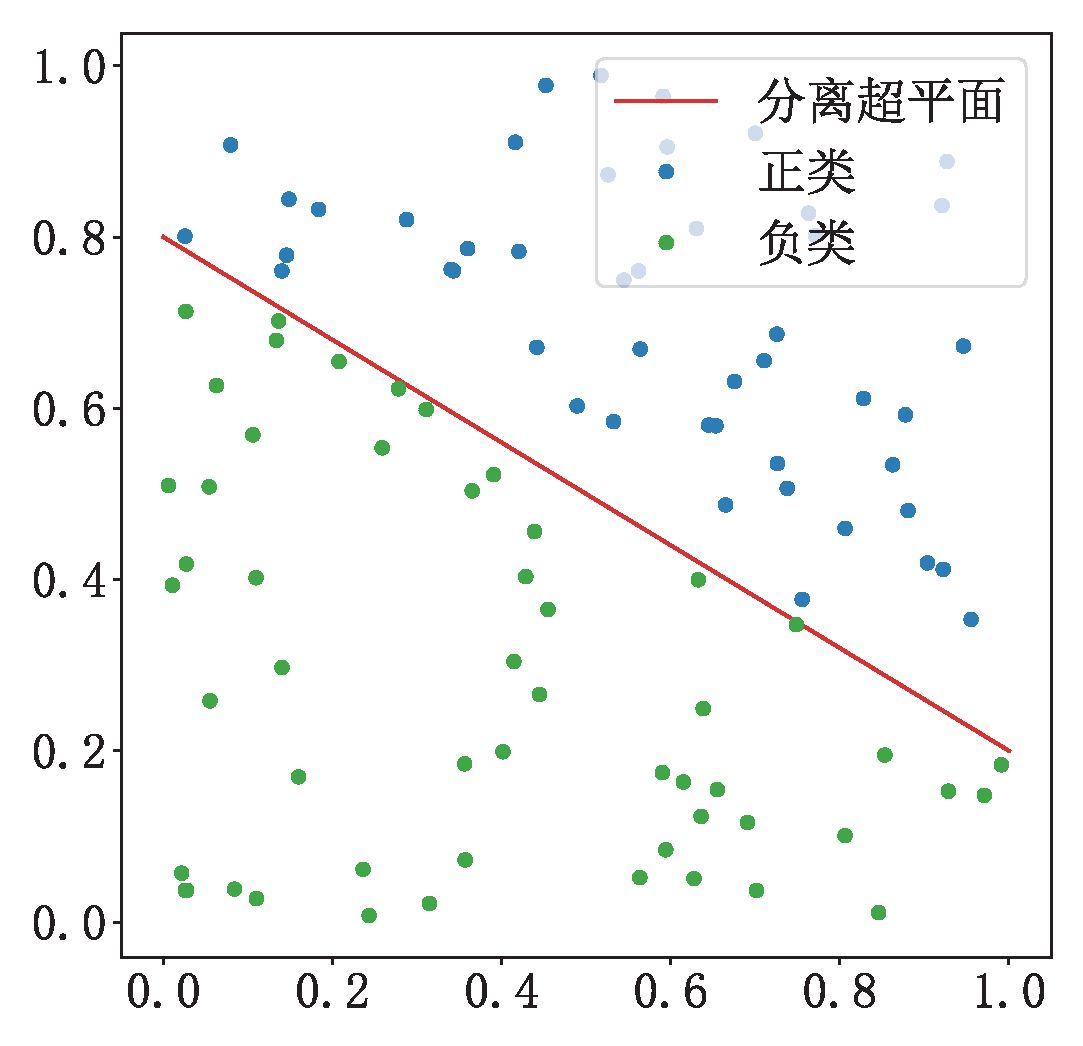
\includegraphics[scale=0.5]{分离平面.eps}
    \caption{分离超平面}
    \label{figure-分离超平面}
\end{figure}

\begin{definition}[线性可分性]
    给定一个数据集$T\subset \bR^n$, 如果存在超平面$S: \bd{w}^T\bd{x} + b = 0$, 能够将数据集的正负样本点完全正确的划分到超平面的两侧, 则称该数据集线性可分, 否则线性不可分.
\end{definition}
\subsection{学习准则}
为了描述一个样本集合, 我们定义二元组$(\bd{x},  y)$为一个\textbf{样本(Example)}, 也称为\textbf{实例(Instance)}, $\bd{x}\in\bR^n$称为该样本的\textbf{特征向量(Feature Vector)}, 每一维表示一个\textbf{特征(Feature)}, $y\in\{-1, 1\}$为该样本的\textbf{标签(Label)}(在这里就是该样本对应的分类).给定如下的一个大小为$N$的线性可分的样本集$T$. (比如\textbf{图\ref{figure-分离超平面}} 中的样本集就是一个线性可分的)
\begin{equation}
    \mathcal{T} = \{(\bd{x}^{(1)}, y^{(1)}), (\bd{x}^{(2)}, y^{(2)}), \cdots, (\bd{x^{(N)}}, y^{(N)}):\bd{x}_i\in\bR^n, y_i\in\{-1, 1\}, 1\leqslant i\leqslant N\},
\end{equation}
我们将根据\textbf{训练集(Training Set)}(样本集的子集, 用于训练模型)寻找一个超平面$S: \bd{w}^T\bd{x}+b=0$, 即学习参数$\bd{w}, b$的过程称为\textbf{训练(Training)}, 使其将$T$中的数据完全正确的分离开.因此我们需要制定一个与$\bd{w}$和$b$有关的优化函数, 通过极小化该函数, 从而达到我们的目的, 这里的优化函数在机器学习中被称为\textbf{损失函数(Loss Function)}, 其作用是量化模型预测与真实标签之间的差异, 在整个训练集$\mathcal{T}$上, 我们还可以计算\textbf{经验风险(Empirical Risk)}, 即全体损失函数的平均值. 一种很自然的选取方法是全体误分类点的总数, 但是这样构造的函数并不是连续的, 不易于优化.感知器所选取的损失函数为全体误分类点到超平面$S$的距离之和.

我们知道对于任意的$\bd{x}\in \bR^n$, $\bd{x}$到$S$的距离可以表示为
\begin{equation}
    d = \frac{|\bd{w}^T\bd{x}+b|}{||\bd{w}||},
\end{equation}
其中$||\bd{w}||=\sqrt{w_1^2+w_2^2+\cdots+w_n^2}$ , 即为2-范数.

对于超平面$S$的误分类点$\bd{x}^{(i)}$, 有如下2种情况, 并且可以将它们归为一种: 
\begin{equation}
    \left.\begin{aligned}
    \mathrm{if}\quad y^{(i)}=-1, \quad \bd{w}^T\bd{x}^{(i)}+b > 0\ \\
    \mathrm{if}\quad y^{(i)}=1, \quad \bd{w}^T\bd{x}^{(i)}+b<0\ 
    \end{aligned}\right\}\ 
    y^{(i)}(\bd{w}^T\bd{x}^{(i)}+b)<0.
\end{equation}

则$\disp |\bd{w}^T\bd{x}^{(i)}+b| = -y^{(i)}(\bd{w}^T\bd{x}^{(i)}+b)$, 因此$\bd{x}^{(i)}$到$S$的距离为
\begin{equation}
    d_i = -\frac{y^{(i)}(\bd{w}^T\bd{x}^{(i)}+b)}{||\bd{w}||},
\end{equation}
不考虑系数$\disp\frac{1}{||\bd{w}||}$, 得感知器损失函数与经验风险函数
\begin{equation}\label{perceptron_loss}
    \L(\bd{x}, y;\bd{w}, b)=\max(0, -y(\bd{w}^T\bd{x}+b)),
\end{equation}
\begin{equation}\label{perceptron_risk}
    \mathcal{R}(\bd{w}, b)=\frac{1}{N}\sum_{i=1}^N\L(\bd{x^{(i)}}, y^{(i)}; \bd{w}, b).
\end{equation}

这里不考虑$\disp\frac{1}{||\bd{w}||}$的原因, 我们认为有如下2个原因: 
\begin{itemize}
    \item 误分类主要由$\disp -y_i(\bd{w}^T\bd{x}+b)$的正负号来判断, 而$\disp\frac{1}{||\bd{w}||}$对符号没有影响.
    \item 便于计算偏导.
\end{itemize}
\subsection{梯度下降法}
根据损失函数(\ref{perceptron_loss})式可知, 可以将感知器学习算法转化为一下的无约束极小化问题
\begin{equation}
    \min_{\bd{w}\in\bR^n, \ b\in\bR}\L(\bd{x}, y;\bd{w}, b)=\max(0, -y(\bd{w}^T\bd{x}+b)).
\end{equation}

考虑使用最速梯度下降法作为该模型的优化算法, 即取优化函数的负梯度方向作为每次一迭代更新参数的下降方向
\begin{align}
    \frac{\partial \L(\bd{x}, y; \bd{w}, b)}{\partial \bd{w}} =&\ \begin{cases}
        -y\bd{x}, &\quad (\bd{x}, y)\in \mathcal{M},\\
        0, &\quad \mathtt{otherwise}.\\
    \end{cases}\\
    \frac{\partial \L(\bd{x}, y; \bd{w}, b)}{\partial b} =&\ \begin{cases}
        -y, &\quad (\bd{x}, y)\in \mathcal{M},\\
        0, &\quad \mathtt{otherwise}.\\
    \end{cases}
\end{align}
其中$\mathcal{M}$为$\mathcal{T}$中所有误分类点集, 即$\mathcal{M} := \{(\bd{x}, y)\in\mathcal{T}:y(\bd{w}^T\bd{x}+b) < 0\}$, 根据每次迭代更新所用的样本集大小, 可将最速下降法分为以下三种算法。
\subsubsection{批量梯度下降法}
\textbf{批量梯度下降法(Batch Gradient Descent,  BGD)}, 每次使用整个训练集$\mathcal{T}$的样本对参数$\bd{w},  b$进行更新, 即直接对经验风险函数进行最小化:
\begin{equation}
    \bd{w}\leftarrow \bd{w} + \frac{\eta}{N}\sum_{(\bd{x}, y)\in \mathcal{M}}y\bd{x}, \quad b\leftarrow b+\frac{\eta}{N}\sum_{(\bd{x}, y)\in \mathcal{M}}y.
\end{equation}
其中$\eta$在机器学习中被称为\textbf{学习率(Learning Rate)}, 也称为\textbf{步长(Step Size)}, 它可以类比最速下降法中的线性步长因子$\alpha$.

优点: 全训练集所确定的方向能够较好的代表样本总体, 从而更准确地朝极小值所在的方向前进.并且, 当目标函数为凸(非凸)函数时, 该算法一定能收敛到全局(局部)最小值点.

缺点: 每一次迭代需要遍历样本总体, 需花费大量时间, 而且更新是全体样本遍历后发生, 此时部分样本对参数的更新没有太大影响.

\subsubsection{随机梯度下降法}
\textbf{随机梯度下降法(Stochastic Gradient Descent,  SGD)}, 不同于批量梯度下降法, 随机梯度下降法每次迭代只随机地从训练集$\mathcal{T}$中选取一个样本$(\bd{x}, y)$对参数进行更新: 
\begin{equation}
    \bd{w}\leftarrow \bd{w} + \eta y\bd{x}, \quad b\leftarrow b + \eta y,\qquad \mathrm{if}\quad y(\bd{w}^T\bd{x}+b) < 0.
\end{equation}

优点: 思路简单, 易于实现, 而且由于每次迭代只计算了一个样本上的梯度, 使得每一轮参数更新速度加快.

缺点: 不具有收敛性, 会在极小值附近震荡, 而且单个样本无法代表全体的趋势.

\subsubsection{小批量梯度下降法}\label{section-小批量}
\textbf{小批量梯度下降法(Mini-batch Gradient Descent,  MBGD)}, 介于上述两种算法之间一种算法, 每次迭代使用一个以上而又不是全部的训练样本, MBGD先从训练集$\mathcal{T}$中\textbf{随机}选出$B$个样本, 称$B$\textbf{批次大小(batch size)}, 构成集合$\mathcal{B}=\{\bd{x}^{(i_1)}, \cdots, \bd{x}^{(i_B)}\}\subset \mathcal{T}$, 对参数进行更新: 
\begin{equation}
    \bd{w}\leftarrow \bd{w} + \frac{\eta}{B}\sum_{(\bd{x}, y)\in \mathcal{B}\cap \mathcal{M}}y\bd{x}, \quad 
    b\leftarrow b + \frac{\eta}{B}\sum_{(\bd{x}, y)\in \mathcal{B}\cap \mathcal{M}}y.
\end{equation}

优点: 计算速度比BGD快, 收敛速度快, 而且收敛结果更接近BGD的结果.

缺点: 最终结果会在极小值领域内震荡, 而且学习率和批次大小不易于选择.

\subsection{算法实现}

在感知器算法中, 由于参数较少, 损失函数易收敛, 我们选择简单易行的随机梯度下降法作为优化算法, 该算法流程如下: 

\begin{algorithm}[感知器参数学习算法]\label{algorithm-感知器}\ 

步1. 设置最大迭代次数$N$, 学习率$\eta$, 随机初始化$\bd{w}_0,  b_0$, 记$k:= 0$.

步2. 若达到最大迭代次数或训练集中没有误分类点, 停止.

步3. 随机选取样本$(\bd{x}^{(i)},  y^{(i)})\in T$, 若$y^{(i)}(\bd{w}^T\bd{x}^{(i)}+b)\leqslant 0$, 即该样本为误分类点, 计算$\bd{w}_{k+1}\leftarrow \bd{w}_{k} + \eta y^{(i)}\bd{x}^{(i)}, \ b_{k+1}\leftarrow b_{k} + \eta y^{(i)}$.

步4. $k:= k+1$, 转步2.

\end{algorithm}

下面给出感知器核心部分的Python代码, 完整代码请见\textbf{附录\ref{appendix-Perceptron}}, 代码中为了方便存储优化参数, 使用了式(\ref{eq-分类函数})的简写方法, 即$\bd{w}$为增广权重向量.

\pythonfile{../Python/Perceptron_part.py}

\begin{wrapfigure}[13]{l}{.5\linewidth}
    \centering
    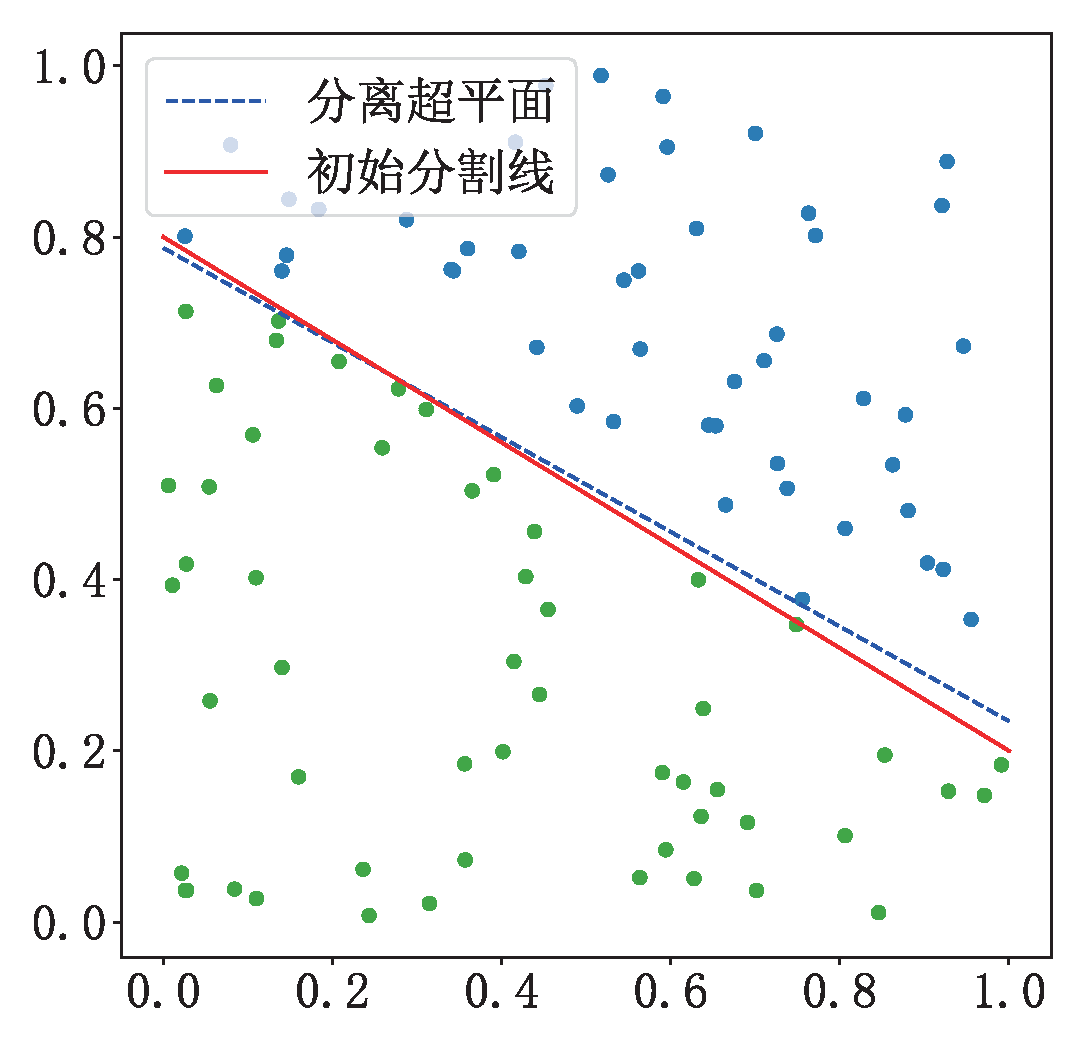
\includegraphics[scale=0.4]{对比图.eps}
    \caption{对比图}
    \label{figure-对比图}
\end{wrapfigure}
\ \newline
为了验证该算法的正确性, 我们先在二维平面$[0,1]\times[0,1]$上随机生成$100$个点, 然后先取定一条分割线, 将整个点集分为两半, 令分割线上方点对应为正类$+1$, 下方点对应为负类$-1$. 然后将这些点作为训练集, 对感知器训练, 学习过程请见\textbf{附录\ref{appendix-迭代过程图}}, 并将最后感知器计算的分离超平面与初始分割线进行对比(如左图\textbf{图\ref{figure-对比图}}).
\newline
\newline
\newline
\newline
\subsection{感知器的收敛性}
对于线性可分的训练集$\mathcal{T} = \left\{(\bd{x}^{(n)}, y^{(n)})\right\}_{n=1}^N$, 其中$\bd{x}^{(n)}$为样本的增广特征向量, 则存在一个正常数$\gamma\ (\gamma > 0)$和增广权重向量$\wtd{\bd{w}}\ (||\wtd{\bd{w}}||^2 = 1)$, 对于任意的$n$均有$y^{(n)}\wtd{\bd{w}}^T\bd{x}^{(n)}\geqslant \gamma$. Novikoff \cite{ref-prove_perceptron}证明了如下定理.
\begin{theorem}[感知器收敛性]
    设$\mathcal{T} = \left\{(\bd{x}^{(n)}, y^{(n)})\right\}_{n=1}^N$为线性可分集, $\gamma$的定义如上, 令$R$为训练集中最大的特征向量的模, 即
    \begin{equation*}
        R = \max_{n}||x^{(n)}||.
    \end{equation*}
    则算法\ref{algorithm-感知器}权重更新次数不超过$\disp \frac{R^2}{\gamma^2}$.
\end{theorem}
\begin{proof}
    感知器算法的更新方法为
    \begin{equation}
        \bd{w}_k = \bd{w}_{k-1}+y^{(k)}\bd{x}^{(k)},
    \end{equation}
    其中$(\bd{x}^{(k)}, y^{(k)})$表示第$k$个分类错误的样本.

    由于初始权重向量$\bd{w}_0 = 0$, 所以在第$n$次更新权重向量时, 有
    \begin{equation}
        \bd{w}_n = \sum_{k=1}^ny^{(k)}\bd{x}^{(k)}.
    \end{equation}
    分别估计$||\bd{w}_k||^2$的上下界:
    \begin{align}
        ||\bd{w}_n||^2 =&\ ||\bd{w}_{n-1}+y^{(n)}\bd{x}^{(n)}||^2 = ||\bd{w}_{n-1}||^2+||y^{(n)}\bd{x}^{(n)}||^2+2y^{(n)}\bd{w}_{n-1}^T\bd{x}^{(n)}\nonumber\\
        \label{eq-proof_perceptron1}\leqslant &\ ||\bd{w}_{n-1}||^2+R^2\leqslant ||\bd{w}_{n-2}||^2+2R^2\leqslant\cdots\leqslant ||\bd{w}_0||^2+nR^2 = nR^2.
    \end{align}
    \begin{align}
        \label{eq-proof_perceptron2}||\bd{w}_n||^2=||\wtd{\bd{w}}||^2||\bd{w}_n||^2\geqslant ||\wtd{\bd{w}}^T\bd{w}_n||^2 = \left|\left|\sum_{k=1}^n\wtd{\bd{w}}^T\left(y^{(k)}\bd{x}^{(k)}\right)\right|\right|^2\geqslant n^2\gamma^2.
    \end{align}

    由公式(\ref{eq-proof_perceptron1})和公式(\ref{eq-proof_perceptron2}), 得到
    \begin{equation*}
        n^2\gamma^2\leqslant ||\bd{w}_n||^2\leqslant nR^2\ \Rightarrow\ n\leqslant \frac{R^2}{\gamma^2}
    \end{equation*}
    因此, 算法\ref{algorithm-感知器}会在$\disp \frac{R^2}{\gamma^2}$步内收敛.
\end{proof}

\subsection{更多的线性模型}
\begin{figure}[h]
    \centering
    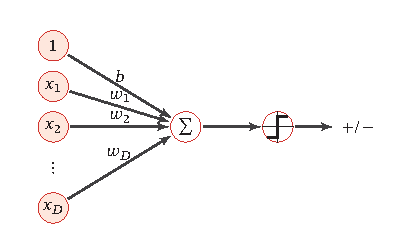
\includegraphics[width=0.5\textwidth]{二分类的线性模型.eps}
    \caption{二分类的线性模型\protect\footnotemark[1]}
    \label{figure-Perceptron}
\end{figure}
\footnotetext[1]{图片来源: 邱锡鹏, 神经网络与深度学习 \cite{ref-qxp}, 第56页}

线性分类模型一般是一个广义的线性函数, 即一个或多个\textbf{线性判别函数}加上一个\textbf{非线性激活函数}, 所谓线性是指决策边界是由一个或多个超平面组成, 常用的分类线性模型除了感知器, 还有支持向量机算法. 回归类问题也可以用于分类模型, 只需将标签值改为对应类别的one-hot向量表示即可, one-hot是对应标签值为$1$其他值为$0$的一种特殊向量. 常用的回归模型有: 线性回归, Logistic回归, Softmax回归.

如果我们将感知器中的激活函数换成其他的非线性函数, 则可以把它视为一个单独的\textbf{神经元}, 再将它们进行堆叠、紧密连接在一起, 就可以形成\textbf{人工神经网络}模型, 该模型可以逼近更加复杂的函数, 对更复杂的数据进行分类, 下文的\textbf{前馈神经网络}就是人们最早发明的一种神经网络结构.

\section{前馈神经网络}
给定一组神经元, 我们可以将神经元作为结点来构造一个网络. 不同的神经网络模型有着不同的网络连接的拓扑结构, 一种比较直接的拓扑结构是前馈网络. \textbf{前馈神经网络(Feedforward Neural Network, FNN)}是最早发明的简单人工神经网络. 前馈神经网络也经常称为\textbf{多层感知器(Multi-Layer Perceptron, MLP)}, 但细节上还是有写区别的, 前馈神经网络是由多层连续的非线性函数构成的, 而不是感知器中不连续的非线性函数构成.

在前馈型神经网络中, 每个神经元都被分到不同层中, 每一层的神经元可以接受到前一层所有神经元所输出的信号, 并产生信号输出到下一层. 我们将第$0$层称为\textbf{输入层}, 最后一层称为\textbf{输出层}, 其他中间层称为\textbf{隐藏层}. 整个网络无反馈, 信号从输入层单向传播到输出层, 整个前馈神经网络也可以用一个无环图来表示. 例如, 图\ref{figure-前馈神经网络}给出了一个三层的前馈神经网络(计算层数时一般不考虑输入层).

\begin{figure}[htbp]
    \centering
    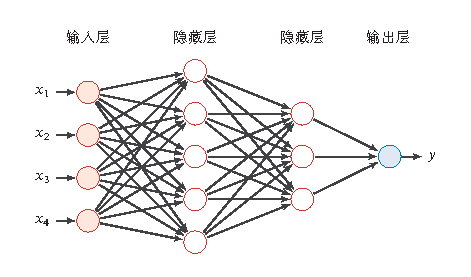
\includegraphics[scale=1.5]{前馈神经网络.eps}
    \caption{前馈神经网络\protect\footnotemark[1]}
    \label{figure-前馈神经网络}
\end{figure}
\footnotetext[1]{图片来源: 邱锡鹏, 神经网络与深度学习 \cite{ref-qxp}, 第92页}

\subsection{前馈传播形式}

我们从一个更简单的前馈神经网络(图\ref{figure-计算单个神经元激活值})来看如何计算神经网络中一个神经元的输入信号. 对于第$1$层从上至下第$2$个神经元, 我们将它的净活性值(也称净输入)记为$z_2^{(1)}$, 于是
\begin{equation}\label{eq-计算单个神经元}
    z_2^{(1)} = x_1w_{21}^{(1)} + x_2w_{22}^{(1)} + \cdots + x_mw_{2n}^{(1)},
\end{equation}
我们将第$l$层的输出称为\textbf{活性值(Activation)}$\bd{a}^{(l)}=\left[\begin{matrix}
    a_1^{(l)}&\cdots&a_{N_l}^{(l)}
\end{matrix}\right]^T$, 第$0$层(输入层)的活性值定义为训练样本的特征向量$\bd{x}$, 于是式(\ref{eq-计算单个神经元})也可写为
\begin{equation}\label{eq-计算单个神经元1}
    z_2^{(1)} = a_1^{(0)}w_{21}^{(1)} + a_2^{(0)}w_{22}^{(1)} + \cdots + a_m^{(0)}w_{2n}^{(1)}.
\end{equation}

如果我们记第$l$层的神经元数为$N_l$ , 第$l$层的偏置为$\bd{b}^{(l)}=\left[\begin{matrix}
    b_1^{(l)}&\cdots&b_{N_{l}}^{(l)}
\end{matrix}\right]^T$, 第$l$层的\textbf{净活性值(Net Activation)}为$\bd{z}^{(l)}=\left[\begin{matrix}
    z_1^{(l)}&\cdots&z_{N_l}^{(l)}
\end{matrix}\right]^T$, 第$l-1$层到$l$层的权重矩阵为
\begin{equation*}
    \bd{W}^{(l)}=\left[\begin{matrix}
        w_{11}^{(l)}&\cdots&w_{1,N_{l-1}}^{(l)}\\
        \vdots&\ddots&\vdots\\
        w_{N_l,1}^{(l)}&\cdots&w_{N_l,N_{l-1}}^{(l)}
    \end{matrix}\right]_{(N_l\times N_{l-1})}
\end{equation*}

\begin{figure}[t]
    \centering
    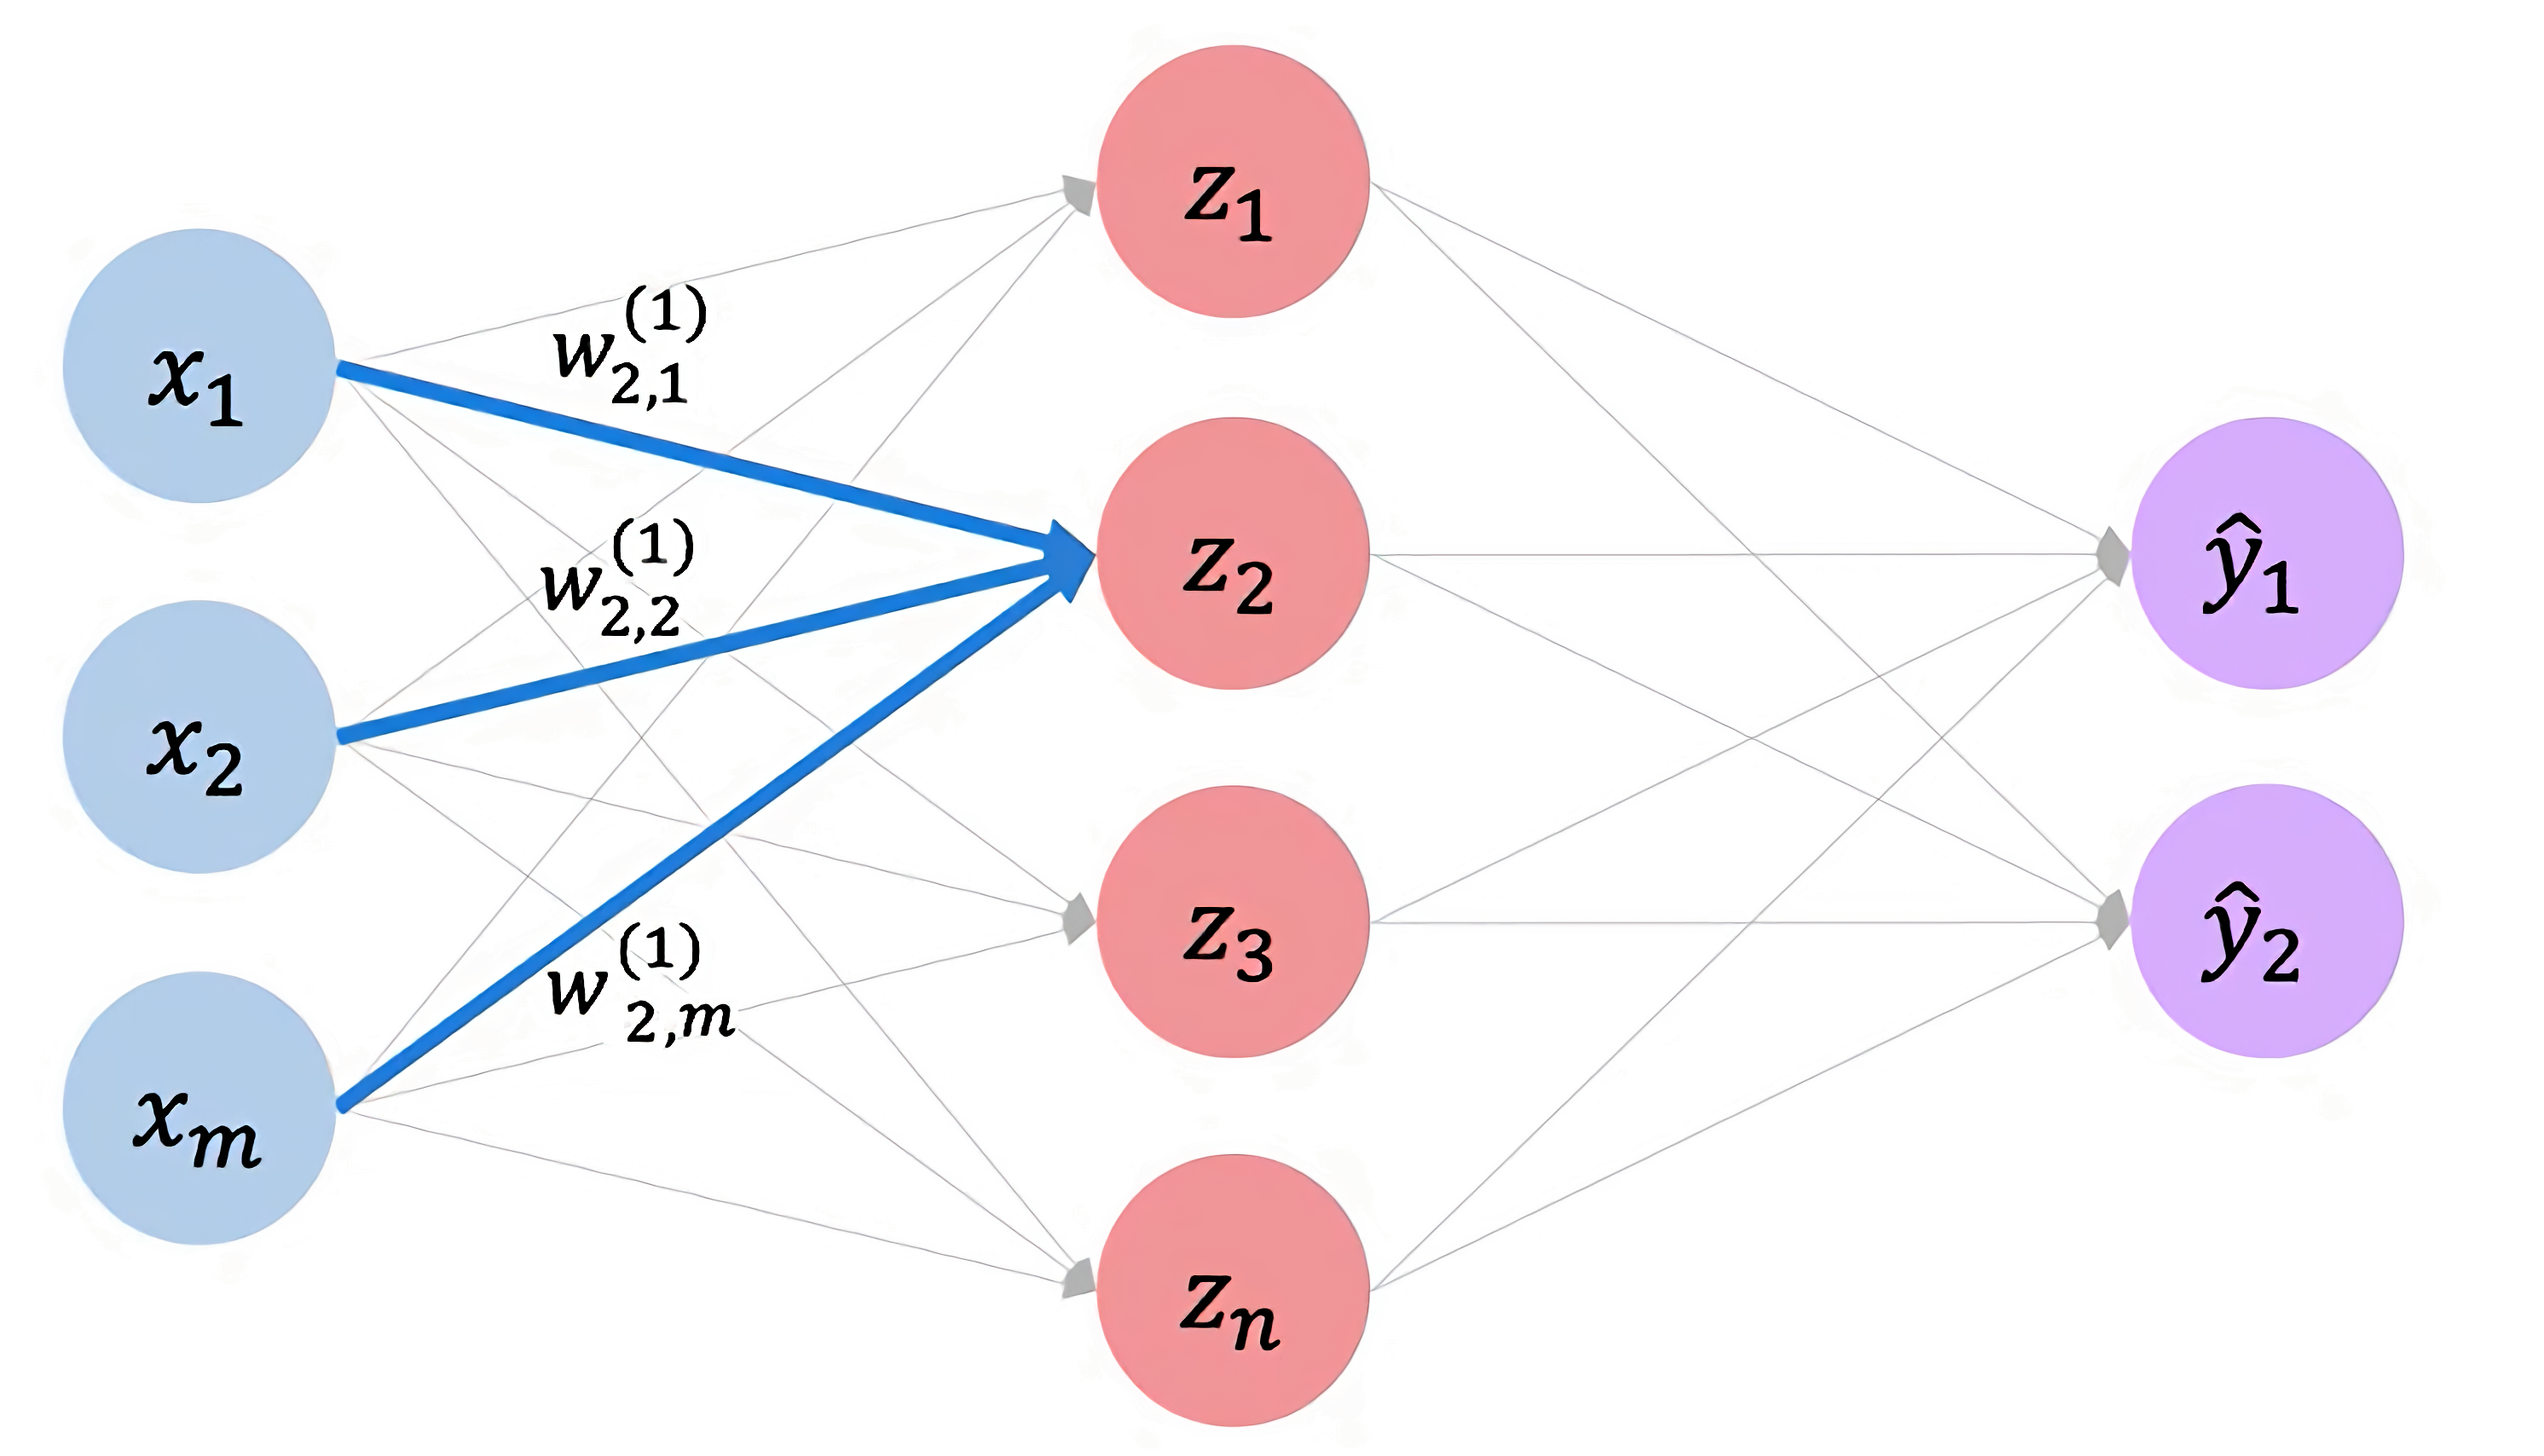
\includegraphics[scale=0.4]{计算单个神经元.png}
    \caption{计算单个神经元激活值\protect\footnotemark[1]}
    \label{figure-计算单个神经元激活值}
\end{figure}
\footnotetext[1]{图片来源: MIT-6S191 \cite{ref-MIT},  Lecture 1 video 24'50''}

根据式(\ref{eq-计算单个神经元1})我们可以写出如下的前馈传播计算公式:
\begin{equation}\label{eq-计算净活性值}
    \bd{z}^{(l)} = \left[\begin{matrix}
        w_{11}^{(l)}&\cdots&w_{1,N_{l-1}}^{(l)}\\
        \vdots&\ddots&\vdots\\
        w_{N_l,1}^{(l)}&\cdots&w_{N_l,N_{l-1}}^{(l)}
    \end{matrix}\right]\left[\begin{matrix}
        a_1^{(l-1)}\\
        \vdots\\
        a_{N_{l-1}}^{(l-1)}
    \end{matrix}\right]+\left[\begin{matrix}
        b_1^{(l)}\\
        \vdots\\
        b_{N_{l}}^{(l)}
    \end{matrix}\right] = \bd{W}^{(l)}\bd{a}^{(l-1)}+\bd{b}^{(l)},
\end{equation}

如果令每一层的神经元的激活函数均为$f_l(\cdot)$, 则
\begin{equation}\label{eq-计算活性值}
    \bd{a}^{(l)} = f_l(\bd{z}^{(l)}),
\end{equation}
首先根据第$l-1$层神经元的\textbf{活性值}$\bd{a}^{(l-1)}$计算出第$l$层神经元的\textbf{净活性值}$\bd{z}^{(l)}$, 然后经过该层的激活函数$f_l(\cdot)$得到第$l$层神经元的\textbf{活性值}.

公式(\ref{eq-计算净活性值})和公式(\ref{eq-计算活性值})可以合并写为:
\begin{equation*}
    \bd{a}^{(l)}=f_l\left(\bd{W}^{(l)}\bd{a}^{(l-1)}+\bd{b}^{(l)}\right),
\end{equation*}
或
\begin{equation}
    \bd{z}^{(l)}=\bd{W}^{(l)}f_{l-1}(\bd{z}^{(l-1)})+\bd{b}^{(l)}.
\end{equation}

这样, 前馈神经网经过逐层的信息传递, 得到最后的输出$\bd{a}^{(L)}$. 整个网络可以看作一个复杂的参数化函数$f(\bd{x}:\bd{W}, \bd{b})$ , 将向量$\bd{x}$作为第$0$层的输入$\bd{a}^{(0)}$, 将第$L$层的输出$\bd{a}^{(L)}$作为整个函数的输出. 信息的传递可以抽象为
\begin{equation}
    \bd{x}=\bd{a}^{(0)}\rightarrow \bd{z}^{(1)}\rightarrow \bd{a}^{(1)}\rightarrow \bd{z}^{(2)}\rightarrow \cdots\rightarrow \bd{a}^{(L-1)}\rightarrow \bd{z}^{(L)}\rightarrow\bd{a}^{(L)}=f(\bd{x};\bd{W},\bd{b}).
\end{equation}
其中$\bd{W},\bd{b}$表示网络中所有层的连接权重和偏置.

下表\ref{table-前馈神经网络}给出了描述前馈神经网络的记号.
\renewcommand\arraystretch{1}
\begin{table}[!htbp] % table标准
    \centering % 表格居中
    \caption{前馈神经网络的记号}\label{table-前馈神经网络}
    \begin{tabular}{p{4cm}p{7cm}} % 设置表格宽度
    %\begin{tabular}{cccc}
        \toprule
        记号 & 含义\\
        \midrule
        $L$ & 神经网络的层数(一般不考虑输入层)\\
        $N_l$ & 第$l$层神经元的个数\\
        $f_l(\cdot)$ & 第$l$层神经元的激活函数\\
        $\bd{W}^{(l)}\in\bR^{N_l\times N_{l-1}}$ & 第$l-1$层到$l$层的权重矩阵\\
        $\bd{b}^{(l)}\in\bR^{N_l}$ & 第$l-1$层到第$l$层的偏置\\
        $\bd{z}^{(l)}\in\bR^{N_l}$ & 第$l$层神经元的净输入(净活性值)\\
        $\bd{a}^{(l)}\in\bR^{N_l}$ & 第$l$层神经元的输出(活性值)\\
        \bottomrule
    \end{tabular}
\end{table}
\subsection{损失函数}
\textbf{损失函数(Loss Function)}是一个用来量化模型预测与真实标签之间的误差, 所以也称为\textbf{误差函数(Error Function)}. 下面介绍两种简单的损失函数. 由于模型都具有损失函数, 我们采用一般的参数化函数的记法, 即模型的预测输出为$f(\bd{x};\theta)$.
\subsubsection{平方损失函数}
\textbf{平方损失函数(Quadratic Loss Funtion)}经常用在预测标签$y$为实数的情况, 定义为
\begin{equation}
    \L(y, f(\bd{x}; \theta)) = \frac{1}{2}(y - f(\bd{x};\theta))^2.
\end{equation}
\subsubsection{交叉熵损失函数}
\textbf{交叉熵损失函数(Cross-Entropy Loss Function)}一般用于分类问题, 假设一共有$C$种标签, 即真实标签$y\in\{1,\cdots,C\}$, 模型的输出$f(\bd{x};\theta)\in[0,1]^C$为类别标签的条件概率分布, 即
\begin{equation}
    p(y=c|\bd{x};\theta) = f_c(\bd{x};\theta),
\end{equation}
其中$f_c(\bd{x};\theta)$表示向量$f(\bd{x};\theta)$的第$c$维分量, 并满足
\begin{equation}
    f_c(\bd{x};\theta)\in[0, 1],\qquad \sum_{c=1}^Cf_c(\bd{x};\theta) = 1,
\end{equation}
这表明我们的模型对第$c$中类别标签的预测概率大小为$f_c(\bd{x};\theta)$.

我们用一个$C$维的one-hot向量$\bd{y}$表示真实标签, 若真实标签为$c$, 则只有$\bd{y}$的第$c$维为$1$, 其他元素均为$0$. 则标签向量$\bd{y}$可以看做样本标签的真实概率分布$p_r(\bd{y}|\bd{x})$, 即样本属于第$c$类的概率为$1$, 属于其他概率均为$0$.

对于两个概率分布, 一般可用交叉熵衡量它们的差异. 标签的真实分布$\bd{y}$和模型预测分布$f(\bd{x};\theta)$之间的交叉熵为
\begin{equation}\label{cross-entropy}
    \L(\bd{y}, f(\bd{x};\theta)) = -\bd{y}\log f(\bd{x};\theta) = -\sum_{c = 1}^Cy_c\log f_c(\bd{x};\theta).
\end{equation}

例如一个五分类问题($C=5$), 一个样本标签为$y=4$, 则其真实分布为$\bd{y} = \left[0\ 0\ 0\ 1\ 0\right]^T$, 若模型预测分布为$f(\bd{x};\theta) = \left[0.1\ 0.1\ 0.1\ 0.5\ 0.2\right]^T$, 则它们的交叉熵为
\begin{equation}
    -\left[\begin{matrix}
        0&0&0&1&0
    \end{matrix}\right]\log\left(\left[\begin{matrix}
        0.1&0.1&0.1&0.5&0.2
    \end{matrix}\right]^T\right) = -\log(0.5) = f_c(\bd{x};\theta)
\end{equation}

由于$\bd{y}$为one-hot向量, 所以公式(\ref{cross-entropy})也可写为
\begin{equation}
    \L(y, f(\bd{x};\theta)) = -\log f_y(\bd{x};\theta).
\end{equation}

{
\begin{wrapfigure}[8]{r}{.35\linewidth}
    \centering
    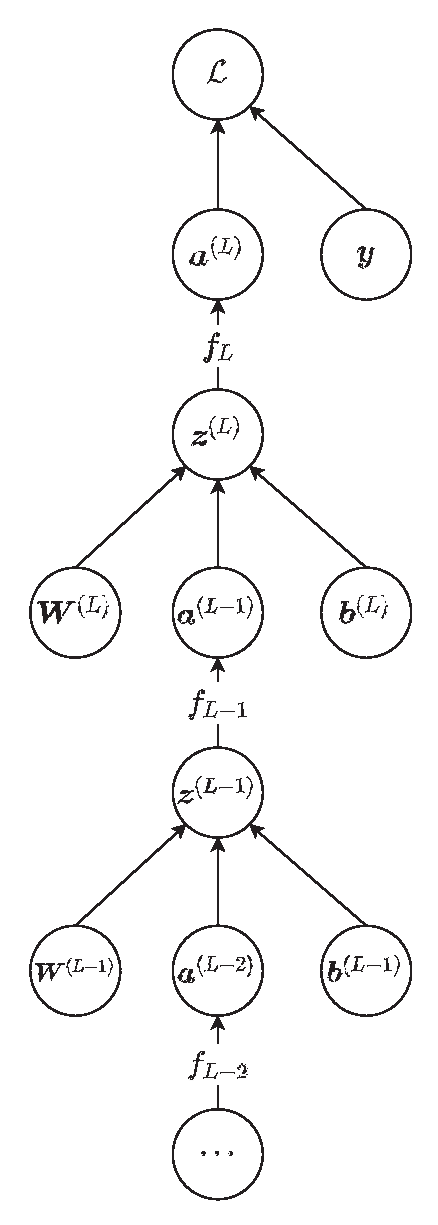
\includegraphics[scale=0.7]{信息传播图.eps}
    \caption{信息传播关系}
    \label{figure-信息传播关系}
\end{wrapfigure}
\subsection{优化算法}
\subsubsection{反向传播算法}
假设采用随机梯度下降法进行神经网络学习, 给定一个样本$(\bd{x}, \bd{y})$, 将其输入到神经网络模型中, 得到网络输出$\wdh{\bd{y}}$. 假设损失函数是$\L(\bd{y}, \wdh{\bd{y}}; \bd{W}, \bd{b})$, 要使用梯度下降法对参数进行学习就需要计算损失函数关于每个参数的偏导数. 

直接单独地对每个参数求偏导数效率太低, 而且非常复杂, 在这里就需要用到神经网络中层与层直接的关系, 逐层求导. 为了更加直观的体现出层与层之间信息传播的关系, 也更加清楚的反映链导法则所涉及的变量, 我们绘制了图\ref{figure-信息传播关系}.

首先从最后一层, 也就是第$L$层开始求偏导, 我们先列出两层参数之间的关系式
\begin{equation}
    \begin{cases}
        \disp z_i^{(l)} = \sum_{j=1}^{N_{l-1}}w_{ij}^{(l)}a_j^{l-1}+b_i^{(l)},\\
        \disp a_i^{(l)} = f_l(z_i^{l}),
    \end{cases}
\end{equation}
其中$w_{ij}^{(l)}$为$\bd{W^{(l)}}$中第$(i,j)$位置的元素, $b_i^{(l)}$为$\bd{b}^{(l)}$中第$i$个分量, $z_i^{(l)},\ a_i^{(l)}$同理.

对第$L$层参数求偏导, 可得
\begin{equation}\label{eq-calc_b}
    \frac{\partial \L}{\partial b_i^{(L)}} = \frac{\partial \L}{\partial a_i^{(L)}}\,\frac{\partial a_i^{(L)}}{\partial z_i^{(L)}}\,\frac{\partial z_i^{(L)}}{\partial b_i^{(L)}} = \frac{\partial \L}{\partial a_i^{(L)}}\,\frac{\partial a_i^{(L)}}{\partial z_i^{(L)}},
\end{equation}
\begin{equation}\label{eq-calc_w}
    \frac{\partial \L}{\partial w_{ij}^{(L)}} = \frac{\partial \L}{\partial a_i^{(L)}}\,\frac{\partial a_i^{(L)}}{\partial z_i^{(L)}}\,\frac{\partial z_i^{(L)}}{\partial w_{ij}^{(L)}} = \frac{\partial \L}{\partial a_i^{(L)}}\,\frac{\partial a_i^{(L)}}{\partial z_i^{(L)}}a_j^{(L-1)},
\end{equation}
}

\begin{equation}\label{eq-calc_a}
    \frac{\partial \L}{\partial a_j^{(L-1)}} = \sum_{i=1}^{N_L}\frac{\partial \L}{\partial a_i^{(L)}}\,\frac{\partial a_i^{(L)}}{\partial z_i^{(L)}}\,\frac{\partial z_i^{(L)}}{\partial a_j^{(L-1)}} = \sum_{i=1}^{N_L}\frac{\partial \L}{\partial a_i^{(L)}}f_L'(z_i^{(L)})w_{ij}^{(L)},
\end{equation}
我们将公式(\ref{eq-calc_b}), 公式(\ref{eq-calc_w}), 公式(\ref{eq-calc_a})写成向量的形式, 则
\begin{equation}\label{eq-L_layer}
    \begin{aligned}
        \frac{\partial \L}{\partial \bd{b}^{(L)}} =&\ f_L'(\bd{z}^{(L)})\circ \frac{\partial \L}{\partial \bd{a}^{(L)}},\\
        \frac{\partial \L}{\partial \bd{W}^{(L)}}=&\ \left(f_L'(\bd{z}^{(L)})\circ \frac{\partial \L}{\partial \bd{a}^{(L)}}\right)\bd{a}^{(L-1)^T},\\
        \frac{\partial \L}{\partial \bd{a}^{(L-1)}}=&\ \bd{W}^{(L)^T}\left(f_L'(\bd{z}^{(L)})\circ \frac{\partial \L}{\partial \bd{a}^{(L)}}\right),
    \end{aligned}
\end{equation}
其中$\bd{A}\circ\bd{B}$表示求矩阵$\bd{A},\ \bd{B}$的\textbf{Hadamard积}, 也就将两个矩阵的对应项相乘. $f_l'(\bd{z}^{(l)})$为按位计算的函数, 即
\begin{equation}
    f_l'(\bd{z}^{(l)}) = \left[\begin{matrix}
        f_l'(z_1)&\cdots&f_l'(z_{N_l})
    \end{matrix}\right]^T,
\end{equation}
$\disp \frac{\partial \L}{\partial \bd{b}^{(l)}}$表示标量对向量的偏导中的\textbf{分母布局(Denominator Layout)}, 即
\begin{equation}
\frac{\partial \L}{\partial \bd{b}^{(l)}} = \left[\begin{matrix}
    \dfrac{\partial \L}{\partial b^{(l)}_1}&\cdots&\dfrac{\partial \L}{\partial b^{(l)}_{N_l}}
\end{matrix}\right]^T\in \bR^{N_l\times 1}.
\end{equation}

不难发现, 公式(\ref{eq-L_layer})中的$L$可以换成任意的$l\ (2\leqslant l\leqslant L)$, 我们称
\begin{equation*}
 \disp \bd{\delta}^{(l)}:=\frac{\partial \L}{\partial \bd{z}^{(l)}} = \frac{\partial \L}{\partial \bd{b}^{(l)}} = f_l'(\bd{z}^{(l)})\circ \frac{\partial \L}{\partial \bd{a}^{(l)}}   
\end{equation*}
为第$l$层神经元的\textbf{误差项(Error)}, 它表示第$l$层神经元对最终损失的影响, 也反映了最终损失对第$l$层神经元的敏感程度. 

公式(\ref{eq-L_layer})可以写为更一般的递推式
\begin{equation}\label{eq-一般递推式}
    \begin{aligned}
        \bd{\delta}^{(l)}=&\ f_L'(\bd{z}^{(l)})\circ \frac{\partial \L}{\partial \bd{a}^{(l)}}=f_L'(\bd{z}^{(l)})\bd{W}^{(l+1)^T}\bd{\delta}^{(l+1)},\\
        \frac{\partial \L}{\partial \bd{b}^{(l)}} =&\ \bd{\delta}^{(l)},\\
        \frac{\partial \L}{\partial \bd{W}^{(l)}}=&\ \bd{\delta}^{(l)}\bd{a}^{(l-1)^T},\\
        \frac{\partial \L}{\partial \bd{a}^{(l-1)}}=&\ \bd{W}^{(l)^T}\bd{\delta}^{(l)},
    \end{aligned}\quad (2\leqslant l\leqslant L)
\end{equation}
为了更好的理解公式(\ref{eq-一般递推式})中定义参数的含义, 我们取$L=4$, 简记$f_l' := f_l(z^{(l)})$, 可得如下关系式
\begin{equation}\label{eq-理解参数含义}
    \frac{\partial \L}{\partial \bd{a}^{(1)}} = \bd{W}^{(2)^T}\cdot \overbrace{f_2'\circ \underbrace{\bd{W}^{(3)^T}\cdot \overbrace{f_3'\circ \underbrace{\bd{W}^{(4)^T}\cdot \overbrace{f_4'\circ \frac{\partial \L}{\partial a^{(4)}}}^{\bd{\delta}^{(4)}}}_{\frac{\partial \L}{\partial \bd{a}^{(3)}}}}^{\bd{\delta}^{(3)}}}_{\frac{\partial \L}{\partial \bd{a}^{(2)}}}}^{\bd{\delta}^{(2)}},
\end{equation}
公式(\ref{eq-理解参数含义})中省略了括号, 计算顺序应为从右至左.

结合公式(\ref{eq-一般递推式})我们给出\textbf{反向传播(BackPropagation, BP)}的递推形式:
\begin{align}
    \text{初始化}:&\ \quad \bd{\delta}^{(L)}=f_L'\circ \frac{\partial \L}{\partial \bd{a}^{(L)}},\\
    \text{递推求解}:&\ \quad \frac{\partial \L}{\partial \bd{b}^{(l)}} = \bd{\delta}^{(l)}, \qquad \frac{\partial \L}{\partial \bd{W}^{(l)}} = \bd{\delta}^{(l)}\bd{a}^{(l-1)^T},\\
    \label{eq-误差反向传播}&\ \qquad \bd{\delta}^{(l-1)} = f_{l-1}'\circ \left(\bd{W}^{(l)^T}\bd{\delta}^{(l)}\right).\quad(2\leqslant l\leqslant L)
\end{align}
从公式(\ref{eq-误差反向传播})可以看出, 第$l$层的误差项可以通过第$l+1$层的误差项计算得到, 这就是误差的\textbf{反向传播}. 其含义是: 第$l$层的一个神经元的误差项(或最终损失对该神经元的敏感度)是所有与该神经元相连的第$l+1$层的神经元误差项的权重和, 然后乘上该神经元激活函数的梯度. 图\ref{figure-传播算法流程图}给出了一个$2$层神经网络结构的整个传播算法流程图.
\begin{figure}[htbp]
    \centering
    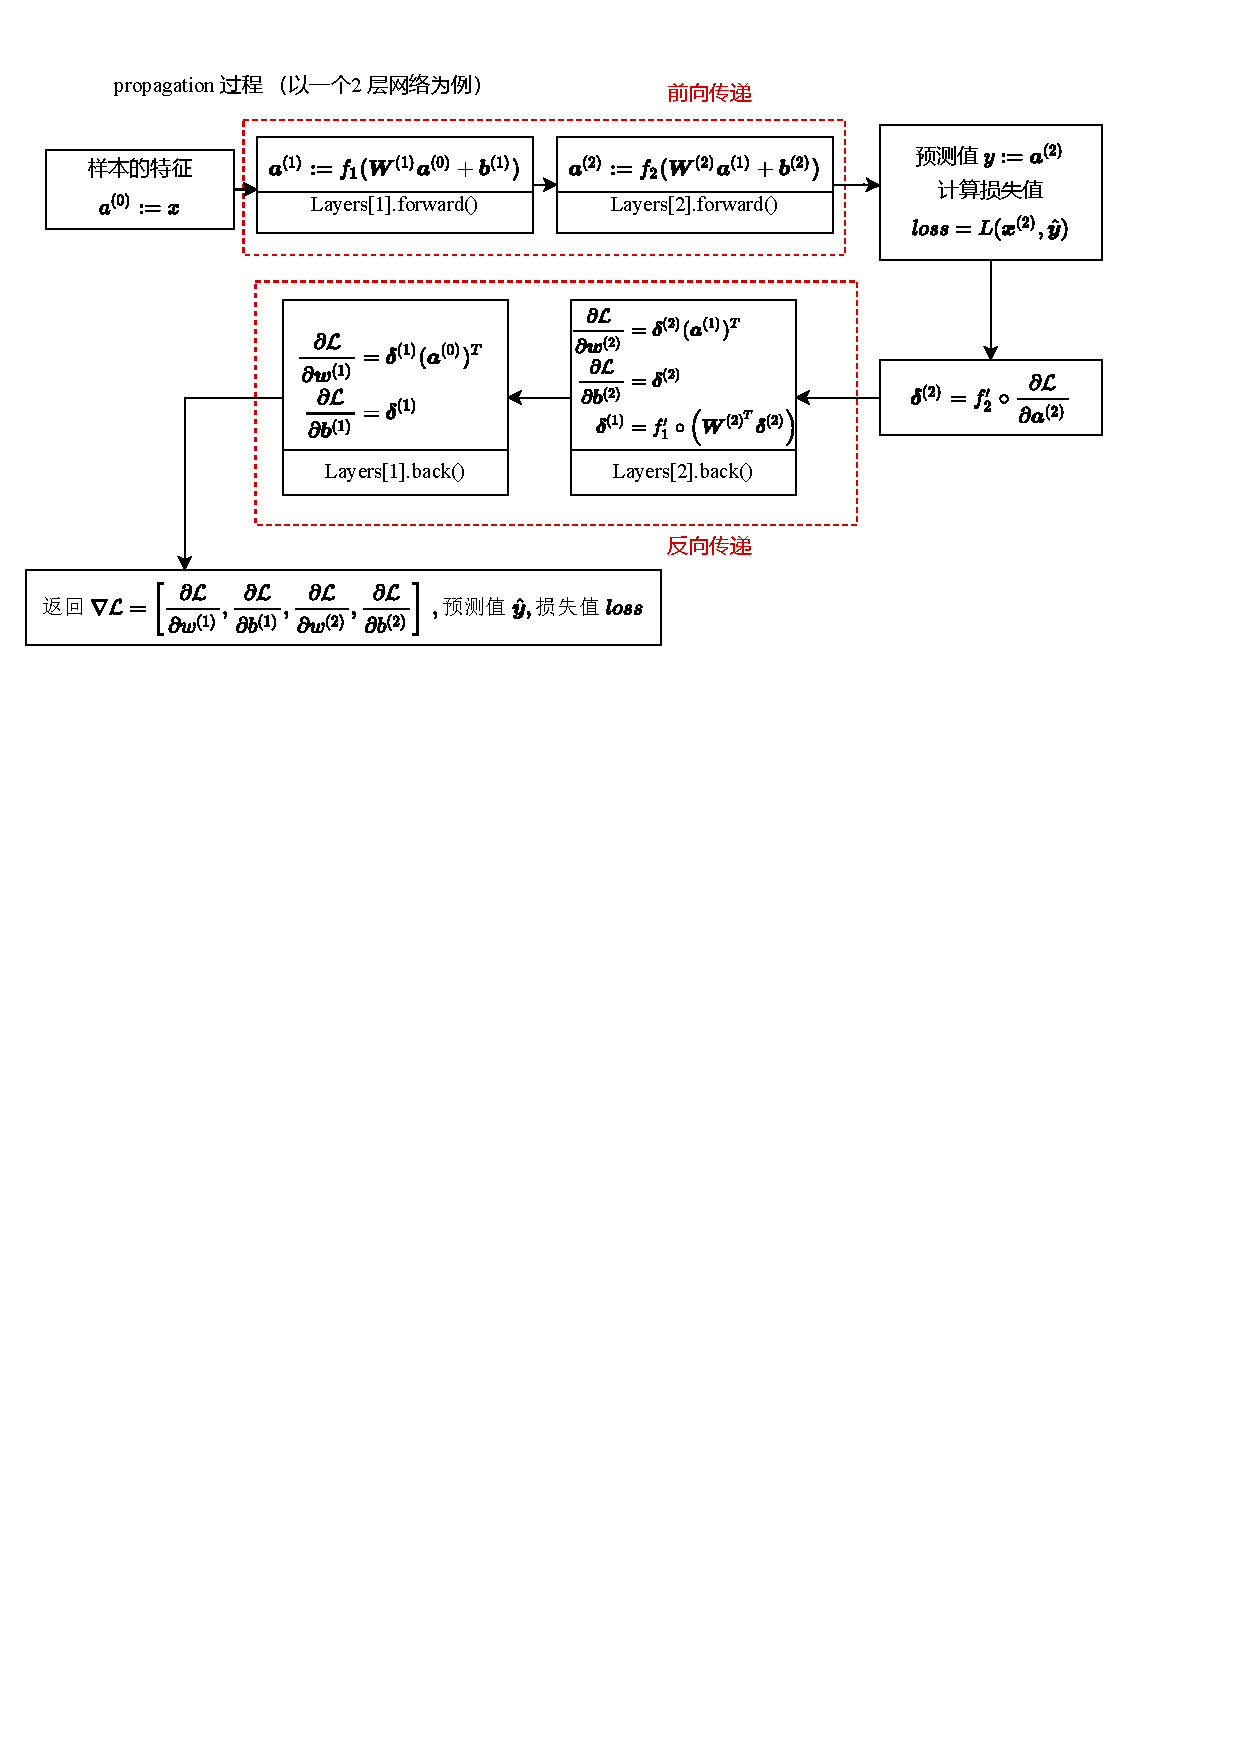
\includegraphics[scale=0.85]{传播算法流程图.pdf}
    \caption{传播算法流程图}
    \label{figure-传播算法流程图}
\end{figure}
\pythonfile{../Python/propagation.py}

\subsection{激活函数}
在前馈神经网络中, 每一层的神经元都有一个激活函数, 为了增强网络的表示能力和学习能力, 激活函数需要具备以下几点性质:

(1) 连续可导(只在一个零测集上不可导)的非线性函数.

(2) 激活函数及其导数应该尽可能简单, 有利于提高网络的计算效率.

(3) 激活函数的导函数应在一个合适的区间内, 否则影响训练的效率和稳定性.
\subsubsection{Sigmoid型函数}
\paragraph{Logistic函数} Logistic函数定义为
\begin{align}
    \sigma(x) =&\ \frac{1}{1+e^{-x}},\\
    \sigma'(x) =&\ \sigma(x)(1-\sigma(x)).
\end{align}

Logistic函数可以看成一个"挤压"函数, 将实数域的驶入"挤压"到$(0,1)$. 当输入值在$0$附近时, Sigmoid型函数近似为线性函数, 当输入值靠近两端时, 对输入进行抑制. 这与生物神经元类似, 对一些输入会产生兴奋, 对另一些输入会产生抑制. 和感知器使用的阶跃函数相比, Logistic函数是连续可导的, 其数学性质更好.

\paragraph{Tanh函数}Tanh函数也是一种Sigmoid型函数. 其定义为
\begin{align}
    \tanh(x) =&\ \frac{e^x-e^{-x}}{e^{x}+e^{-x}},\\
    \tanh'(x) =&\ 1-\tanh^2(x).
\end{align}
Tanh函数可以看作放大并平移的Logistic函数, 其值域是$(-1,1)$.
\begin{equation}
    \tanh(x) = 2\sigma(2x)-1.
\end{equation}

图\ref{figure-函数对比}给出了Logistic函数和Tanh函数的形状. Tanh函数的输出是\textbf{零中心(Zero-Centered)}, 而Logistic函数的输出恒大于$0$. 非零中心化的输出可以使得下一层的神经元的输入发生\textbf{偏置偏移(Bias Shift)}, 并进一步使得梯度收敛速度变慢.

\begin{figure}[htbp]
    \centering
    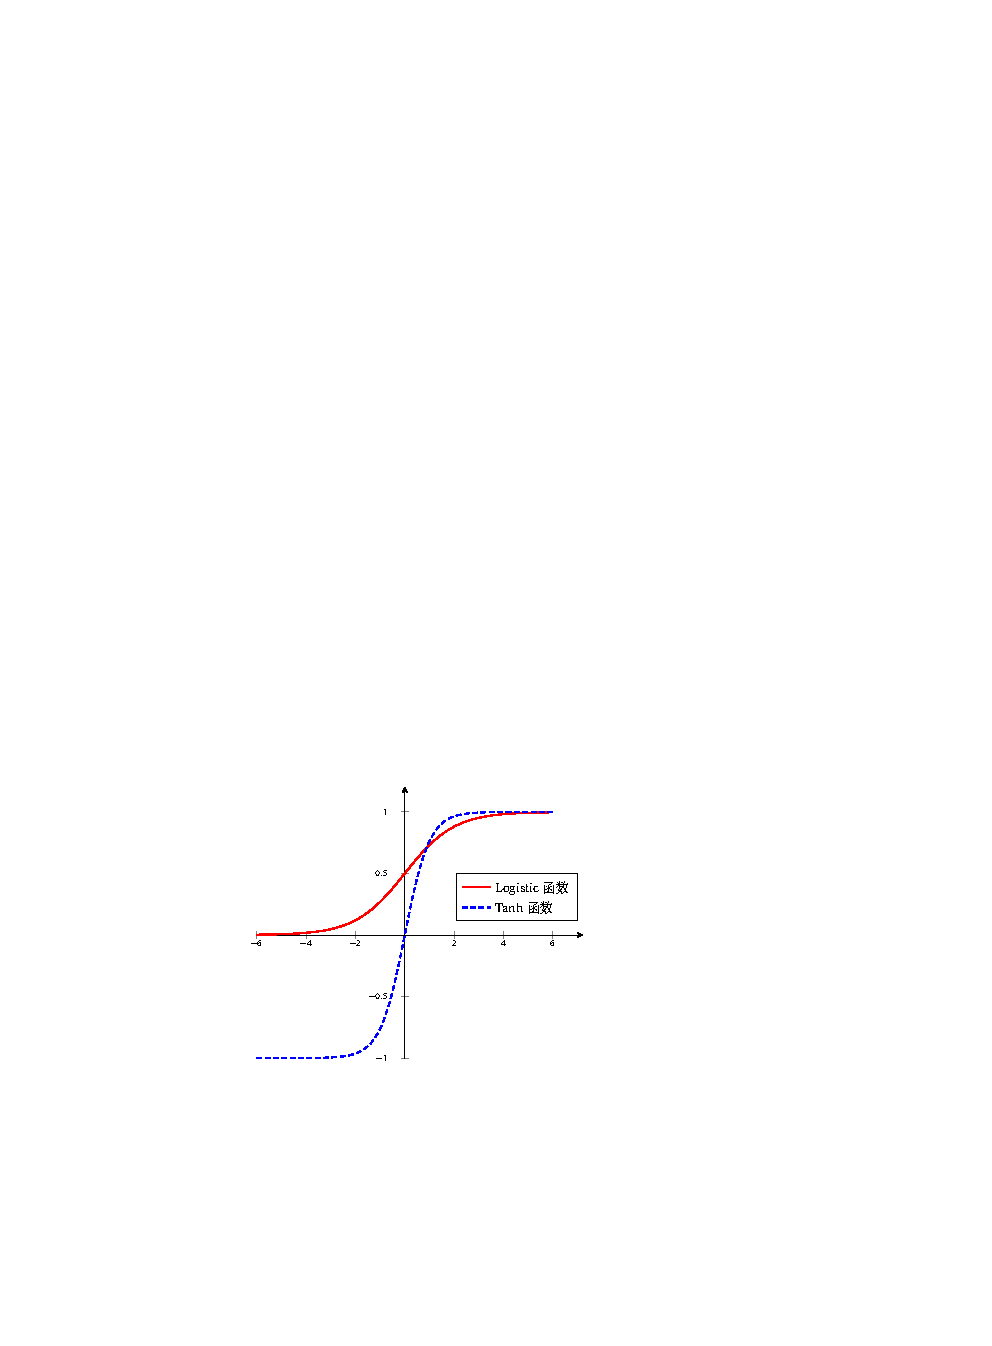
\includegraphics[scale=1.5]{Logistic和Tanh.pdf}
    \caption{Logistic函数和Tanh函数\protect\footnotemark[1]}
    \label{figure-函数对比}
\end{figure}
\footnotetext[1]{图片来源: 邱锡鹏, 神经网络与深度学习 \cite{ref-qxp}, 第84页}
\subsubsection{ReLU函数}\textbf{ReLU(Rectified Linear Unit, 修正线性单元)}, 也称线性整流函数, 是目前深度神经网络中经常使用的激活函数. ReLU实际上是一个斜坡(ramp)函数, 定义为
\begin{equation}
    \text{ReLU}(x) = \begin{cases}
        x,&\quad x \geqslant 0\\
        0,&\quad x < 0
    \end{cases} = \max(0, x).
\end{equation}
\paragraph{优点} ReLU函数形式简单, 只需进行加、乘和比较的操作, 计算上更加高效. ReLU函数也被认为有一定的生物学原理\cite{ref-ReLU}, 例如单侧抑制, 具有高兴奋程度的性质. 同时由于ReLU函数导数唯一, 所以在一定程度上缓解了神经网络的\textbf{梯度消失问题}, 加速了梯度下降的收敛速度.

\paragraph{缺点} 在训练时, 如果参数在一次不恰当更新后, 某一个隐藏层的ReLU函数在训练时在所有训练数据上都不能被激活, 那么这个神经元的梯度永远是0, 以后训练过程中都不会被更新, 这种现象称为\textbf{死亡ReLU问题(Dying ReLU Problem)}. 为了避免这种问题, 引入了\textbf{带泄露的ReLU(Leaky ReLU)}, 即当$x<0$时, 保持一个很小的梯度$\gamma$, 定义如下
\begin{equation}
    \text{LeakyReLU}(x) = \begin{cases}
        x,&\quad x \geqslant 0\\
        \gamma x,&\quad x < 0
    \end{cases} = \max(0, x) + \gamma\min(0, x),
\end{equation}
其中$\gamma$是一个很小的常数.
\begin{figure}[htbp]
    \centering
    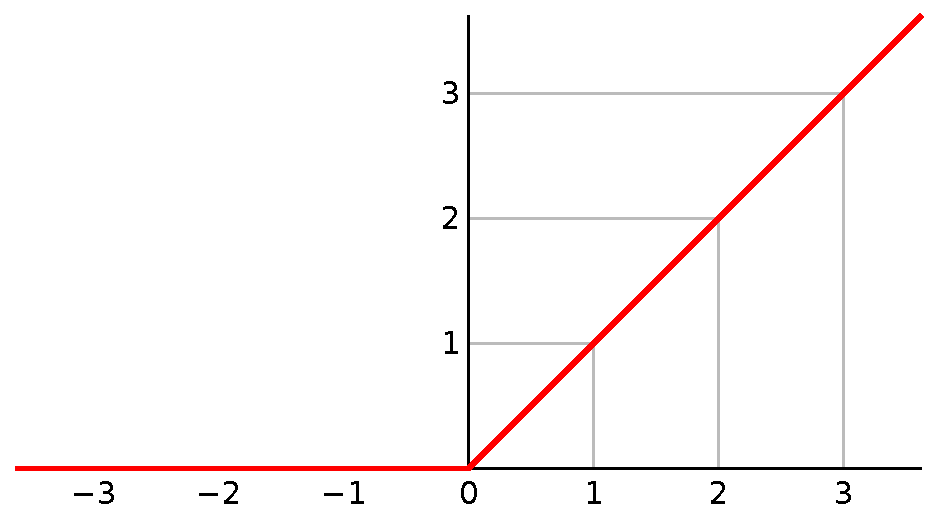
\includegraphics[scale=0.5]{Ramp_function.pdf}
    \caption{ReLU函数\protect\footnotemark[1]}
    \label{figure-Ramp}
\end{figure}
\footnotetext[1]{图片来源: \url{https://zh.m.wikipedia.org/zh-hans/File:Ramp_function.svg}}

\subsection{算法实现}
我们以识别手写数字作为前馈神经网络的应用, 使用小批量随机梯度下降法(\ref{section-小批量}), 使用MNIST数据集, 在\nameref{appendix-Input}中, 我们先将MNIST数据集文件进行解压, 转化为Numpy中array类. 在\nameref{appendix-Main}中, 先将输入的像素数据(范围在$[0, 255]$)正规化处理为$[0,1]$作为样本的特征向量, 样本的标签处理为$\bR^{10\times 1}$的one-hot向量, 若样本的标签为$1$, 则对应的one-hot向量为$[\begin{matrix}
    0&1&0&\cdots&0
\end{matrix}]^T\in \bR^{10\times 1}$, 即对应位为$1$其他位均为$0$的向量. 然后调用\nameref{appendix-ANN}中的Model类构建网络模型, 再使用\pythoninline{Model.fit}函数进入神经网络训练过程.

每次训练开始时, 将数据集打乱, 然后分为多个Mini-Batch, 每次取出一个Mini-Batch进入到\pythoninline{Model.Batch}函数中, 开始处理每个Mini-batch, 如果有多线程的情况(参考C++多线程代码\footnote[2]{吴天阳的博客: \href{https://wty-yy.github.io/posts/2534/}{BP神经网络算法的基本原理及C++实现}}, Python由于功能限制无法实现真正的多线程)可以同时取出多个训练样本, 同时执行\pythoninline{Model.propagation}函数(该传播算法原理图请见图\ref{figure-传播算法流程图}, 其中会调用\pythoninline{Layer.forward}和\pythoninline{Layer.back}函数, 计算损失值). 再将一个Mini-batch中全部训练样本所返回的梯度求平均值, 对神经网络的$\bd{W}, \bd{b}$参数进行一次更新, 返回到\pythoninline{Model.fit}函数中, 接着取出下一个Mini-batch, 再进入到\pythoninline{Model.Batch}进行参数学习, 直到全部的Mini-batch取完, 一次训练结束.

最后使用验证集, 对神经网络的泛用性进行评估, 我们使用\textbf{准确率}的评价指标评判模型对测试集评价分数, \textbf{准确率(Accuracy)}的定义如下:
\begin{equation}
    \mathcal{A} = \frac{1}{N}\sum_{n=1}^NI(\bd{y}^{(n)} = \hat{\bd{y}}^{(n)}),
\end{equation}
其中$I(x)$为指示函数, 当内部条件$x$为真时$I(x) = 1$, 否则$I(x) = 0$. 最后输出该神经网络的准确率, 结束程序. 我们制作了更加直观的前馈神经网络算法流程图便于理解算法的工作原理, 请见下图\ref{figure-前馈神经网络算法}.
\begin{figure}[htbp]
    \centering
    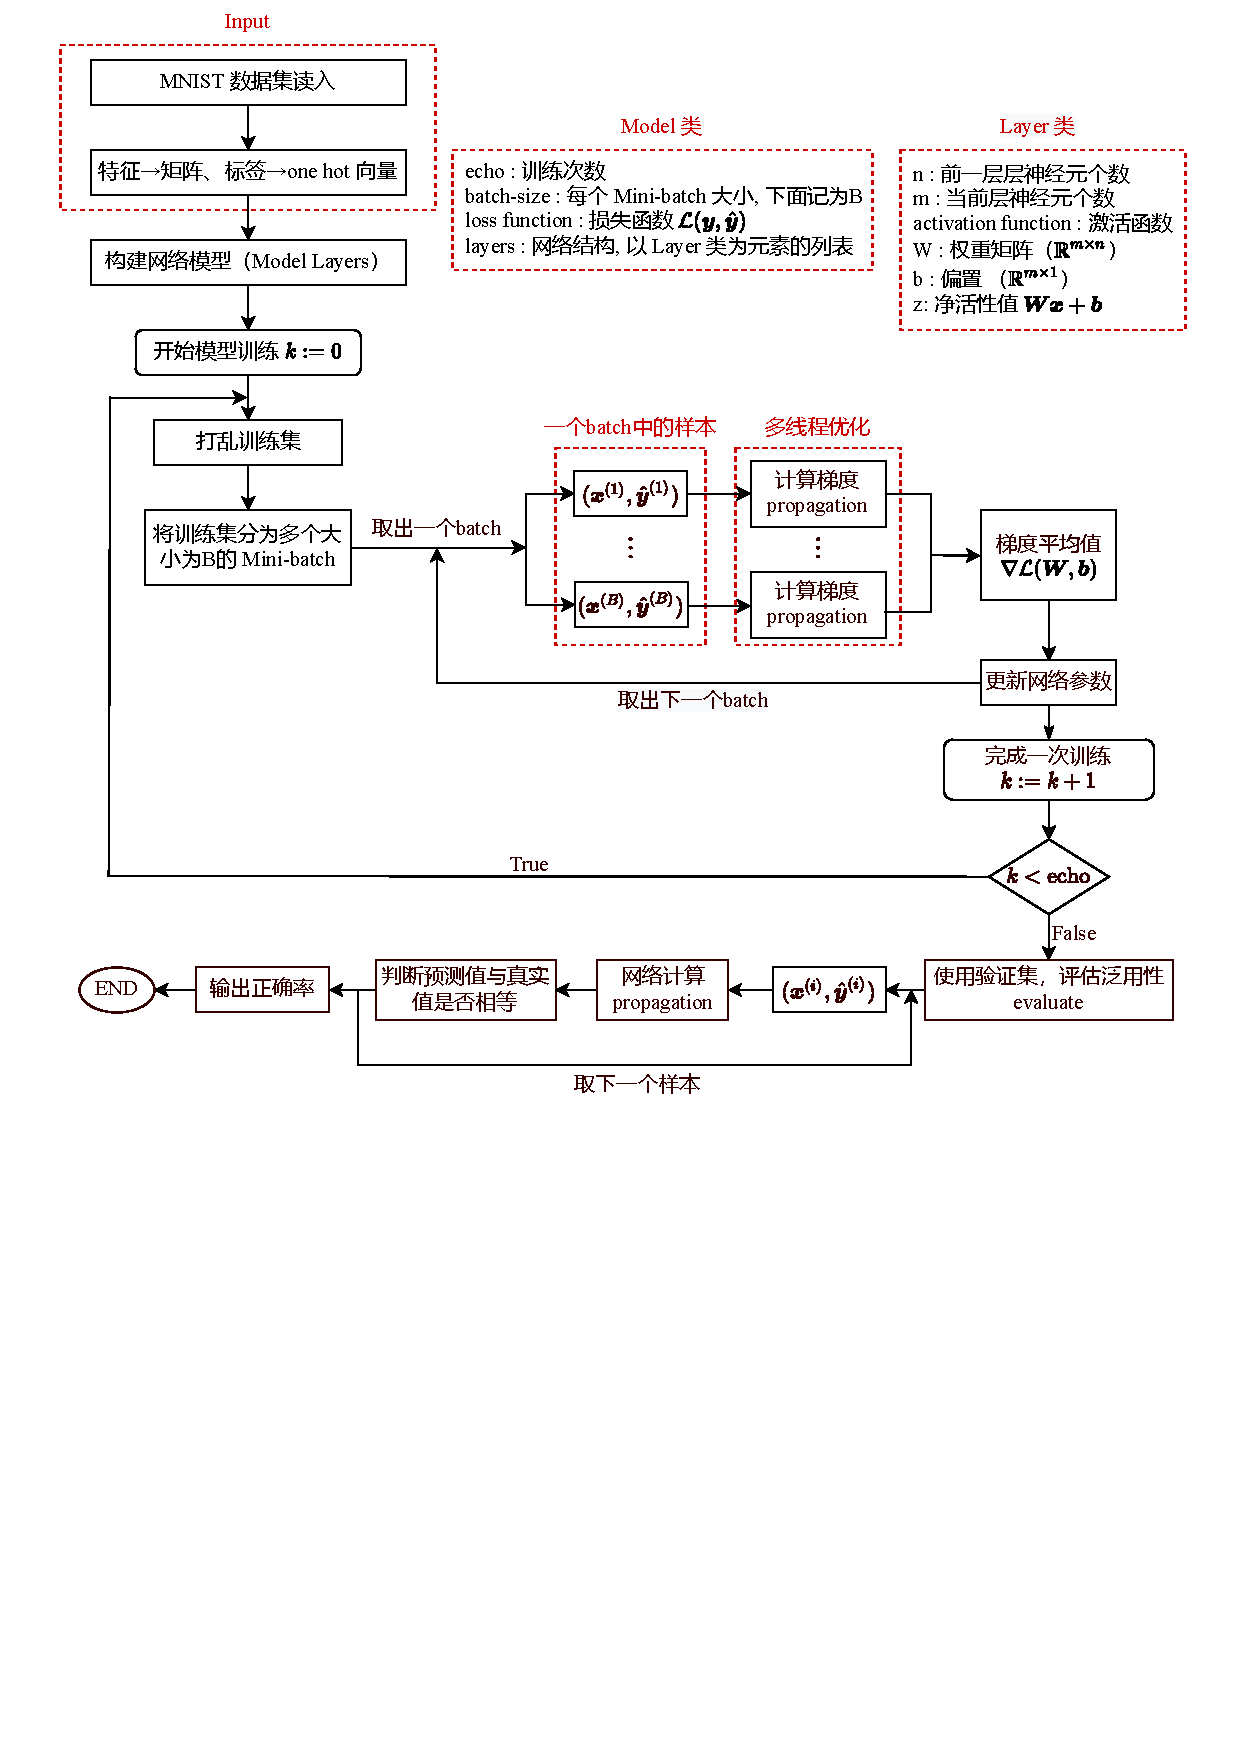
\includegraphics[scale=0.8]{前馈神经网络算法.pdf}
    \caption{前馈神经网络算法流程图}
    \label{figure-前馈神经网络算法}
\end{figure}\del
\subsection{过拟合}
使用梯度下降法的优化算法, 容易发生过拟合现象, 过拟合的定义如下
\begin{definition}[过拟合]
    给定一个假设空间$\mathcal{F}$, 一个假设$f\in\mathcal{F}$, 如果存在其他假设$g\in\mathcal{F}$, 使得在训练集上$f$的损失小于$g$的损失, 但是在整个样本空间上$g$的损失比$f$小, 那么则称假设$f$过度拟合训练数据集.
\end{definition}
为解决过拟合现象, 有如下两种简单的方法.
\subsubsection{提前停止}
由于过拟合的原因, 在训练集上最优的假设$f$, 并不一定是测试集上最优的假设. 因此, 除了训练集和测试集外, 有时会使用一个\textbf{验证集(Validation Set)}来测试模型是否发生了过拟合现象. 在每次迭代时, 将新的模型$f(\bd{x};\theta)$在验证集上进行测试, 计算准确率, 如果在验证集上准确率不再上升, 就停止迭代. 这种策略叫\textbf{提前终止(Early Stop)}. 验证集可以是从训练集中选取一小部分出来, 有时为了方便起见, 也可以将验证集直接取为测试集的一部分.

下图\ref{figure-early_stop}是在识别手写数字中, 网络模型设置为$32$个节点的隐藏层, 使用Sigmoid作为激活函数, Batch Size取为100, 其训练次数与准确率的关系图(这里将验证集随机取为测试集中$10\%$的数据), 并且我们使用了一个$7$阶多项式对真实结果进行拟合, 拟合结果表明在第$51$次训练时准确率接近最大值达到了$0.93$, 后面模型在验证集上的准确率开始缓慢下降, 所以根据提前停止策略应该在$50$次左右停止训练.
\begin{figure}[htbp]
    \centering
    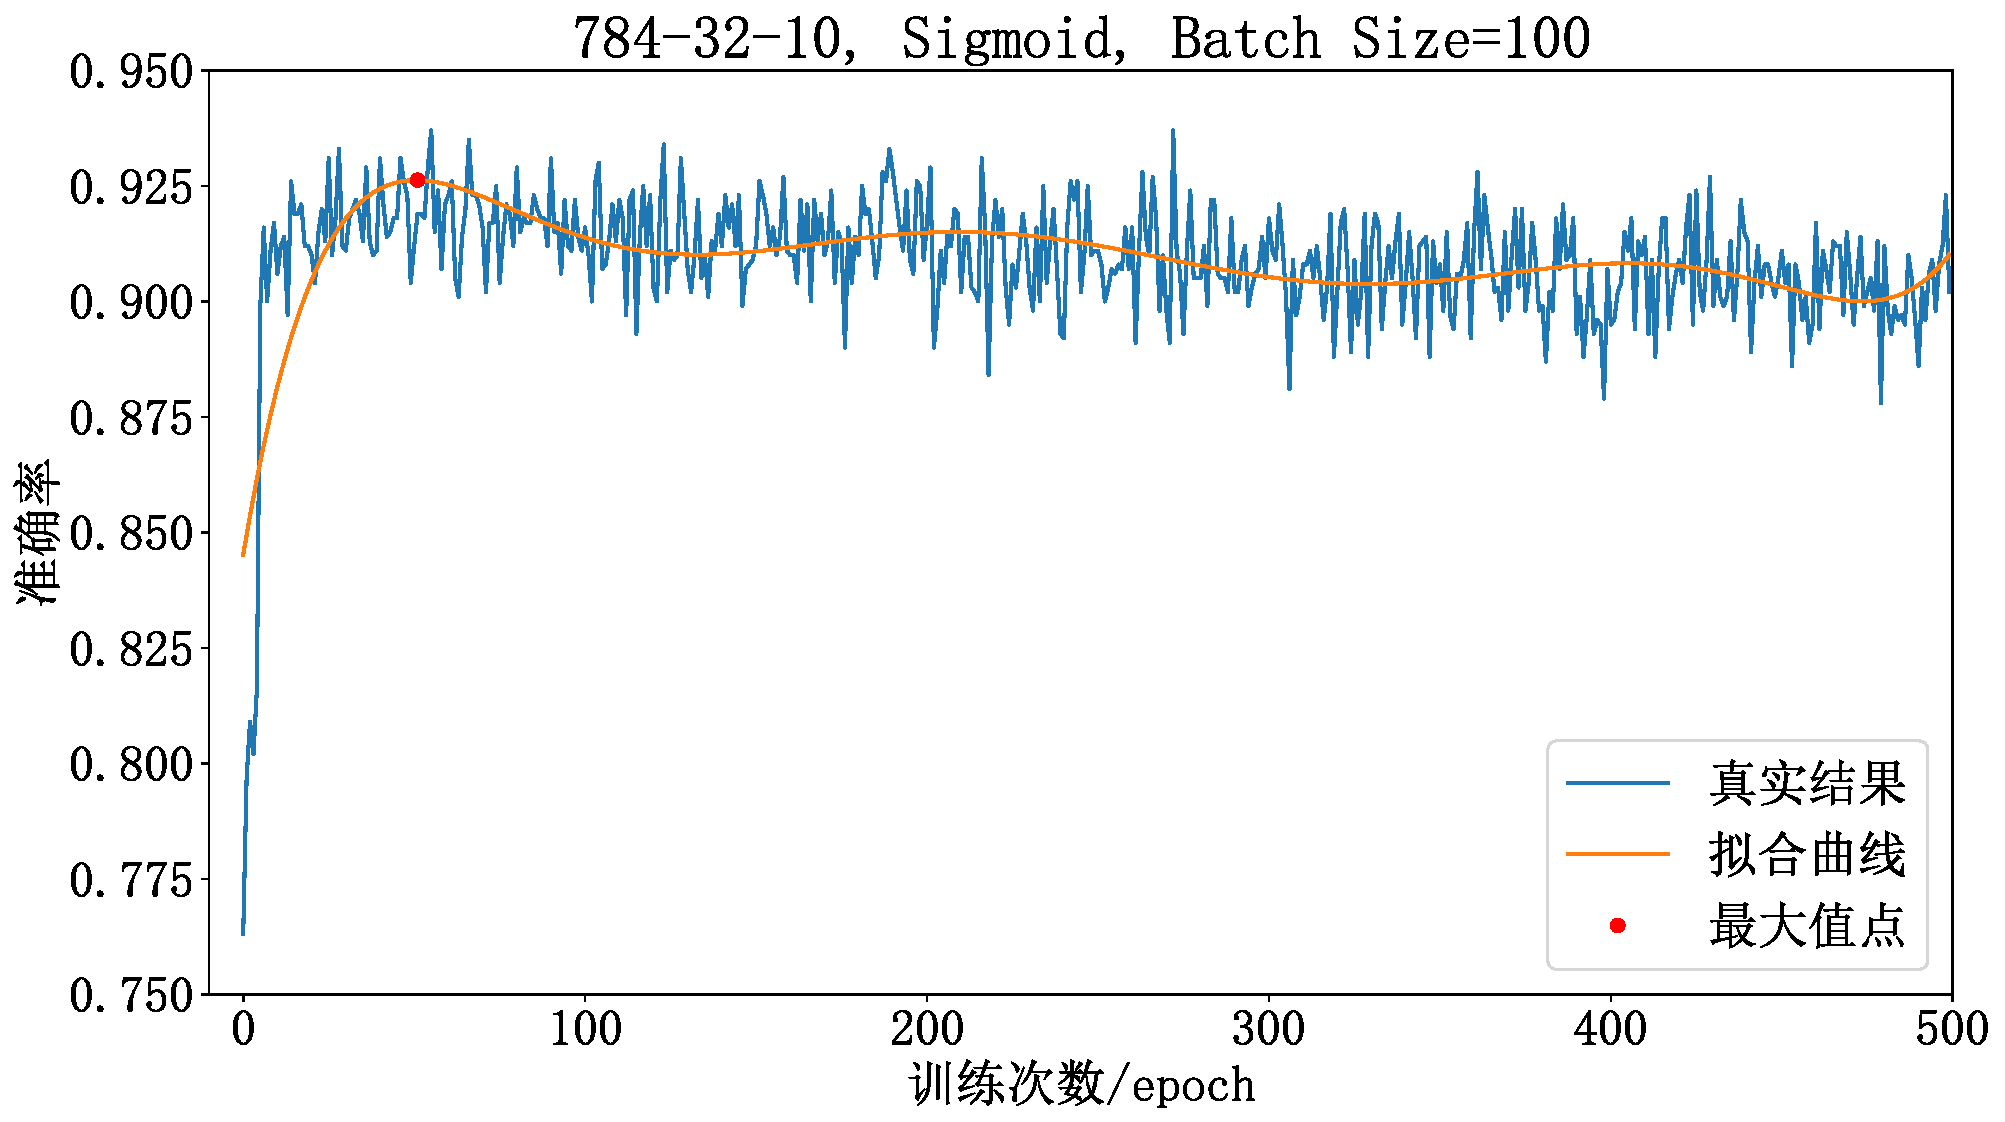
\includegraphics[scale=0.45]{early_stop.pdf}
    \caption{提前终止}
    \label{figure-early_stop}
\end{figure}\del
\subsubsection{丢弃法}
这里还介绍一种简单的方法来避免过拟合, 我们在每次训练网络时丢弃掉一部分的神经元(同时丢弃相连的边), 这种方法称为\textbf{过拟合(Dropout Method)}, 参考Srivastava N, et al.\cite{ref-dropout}. 先设定一个概率$p$, 对每一个神经元都以概率$p$判定是否被丢弃, 只需在计算每一层的活性值时乘上一个选择矩阵即可, 选择矩阵为一个对角阵, 对角线上元素满足概率为$p$的Bernoulli分布. 图\ref{figure-dropout}给出了一个网络应用丢弃法前后的对比图. 

我们尝试将这个方法应用到数字识别中, 但发现效果并不明显, 可能是由于网络节点数目过少或者训练次数太少导致的(也有可能是代码问题), 所以没有对其绘制图像. 根据Hinton G E, et al.\cite{ref-dropout_example}中的结果, 至少使用$800$个节点, 迭代500次以上才能看到明显区别.

\begin{figure}[htbp]
    \centering
    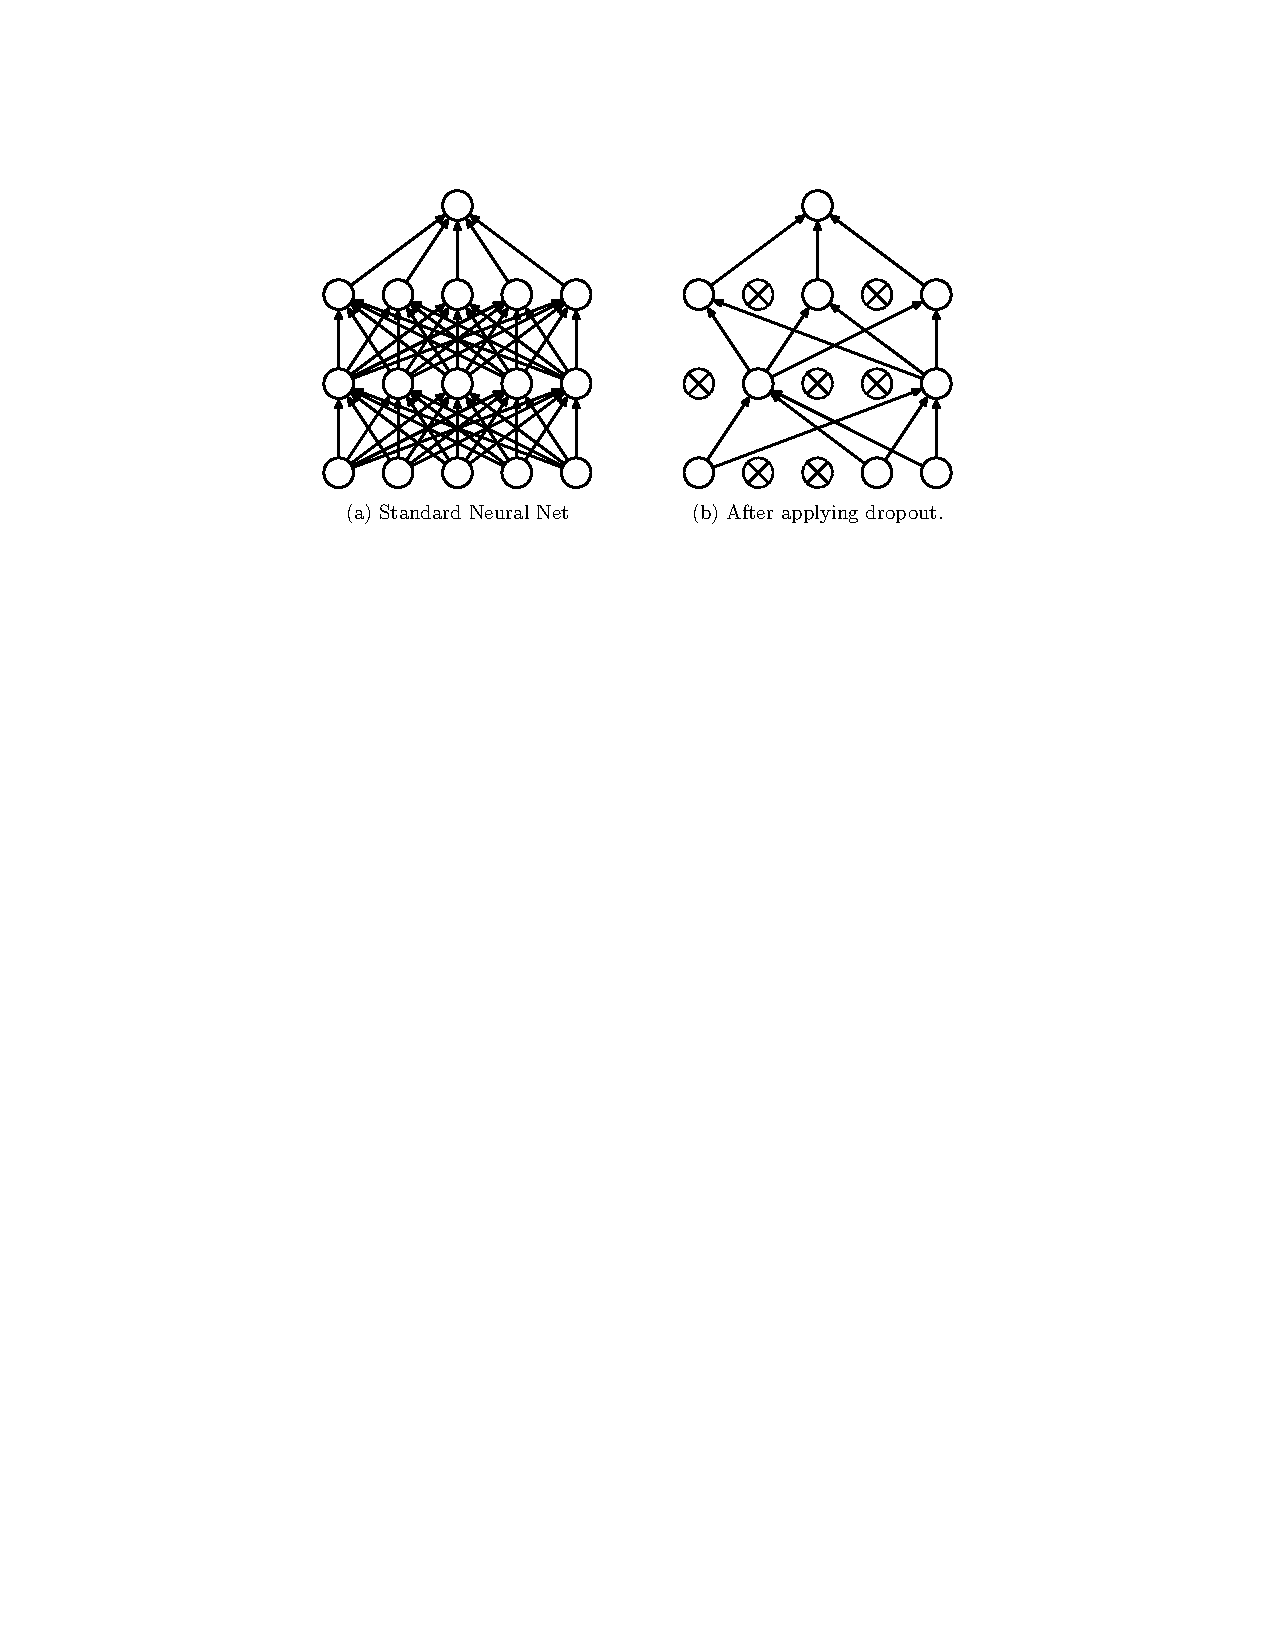
\includegraphics[scale=1]{dropout1.pdf}
    \caption{丢弃法\protect\footnotemark[1]}
    \label{figure-dropout}
\end{figure}
\footnotetext[1]{图片来源: Srivastava N\cite{ref-dropout}, 第2页.}
\subsection{模型参数选择}
我们对手写数字识别的神经网络模型, 固定总训练次数为$500$次, 取$10\%$的测试集作为验证集, 验证每一训练结果的准确率. 通过修改不同的Batch Size大小、网络结构、激活函数, 通过对比得出相对较好网络模型.
\paragraph{Batch Size}
根据图\ref{figure-diff_batch_size}可以看出该模型使用Batch大小为100可以达到较好训练效果, 且训练速度较快.
\begin{figure}[!h]
    \centering
    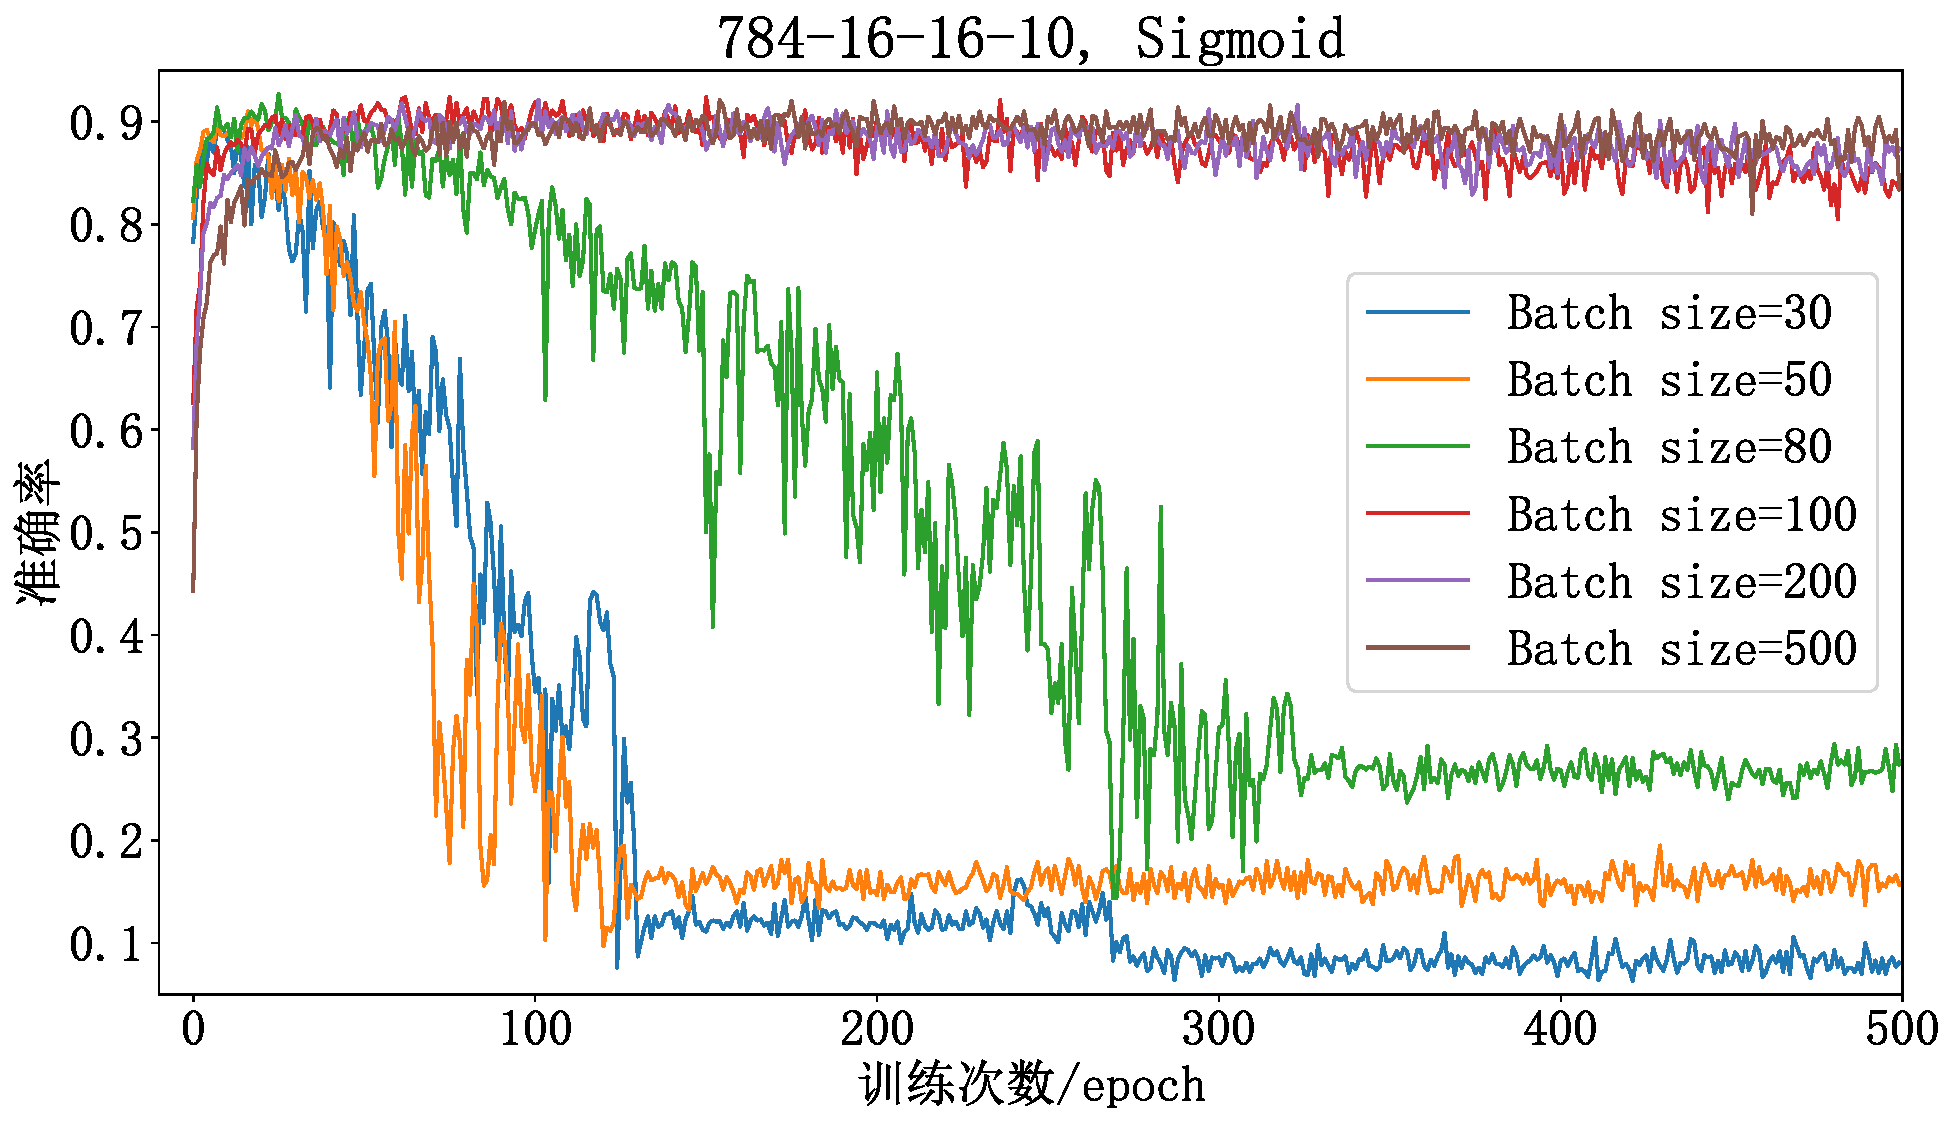
\includegraphics[scale=0.45]{diff_batch_size.pdf}
    \caption{Batch Size对比}
    \label{figure-diff_batch_size}
\end{figure}
\paragraph{网络结构}
根据图\ref{figure-diff_struct}可以看出该模型使用一个含有32个节点的隐藏层网络结构训练效果较好, 且节点数较少, 训练速度更快.
\begin{figure}[htbp]
    \centering
    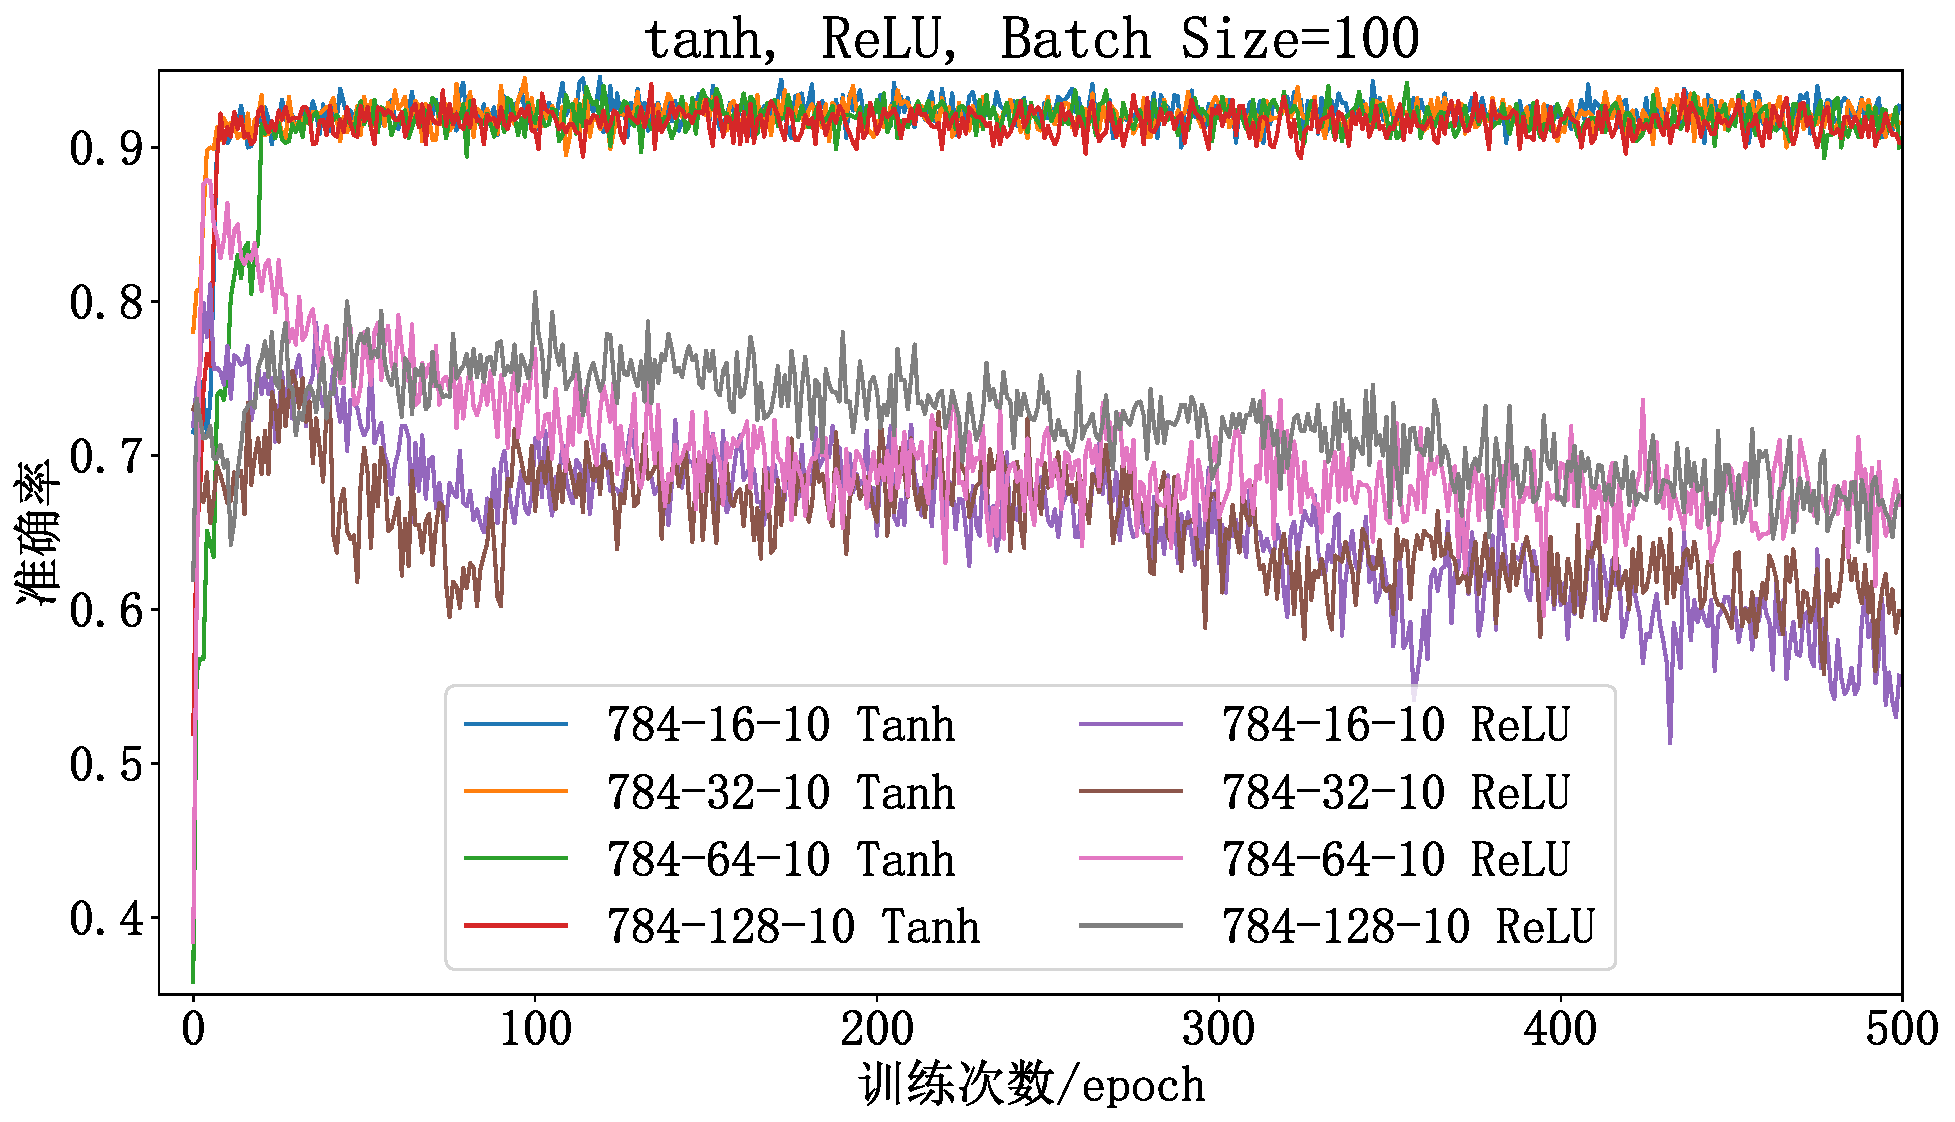
\includegraphics[scale=0.45]{diff_struct.pdf}
    \caption{网络结构对比}
    \label{figure-diff_struct}
\end{figure}\vspace{-2ex}
\paragraph{激活函数}
根据图\ref{figure-diff_activation}可以看出该模型使用Tanh函数训练效果最好.
\begin{figure}[!h]
    \centering
    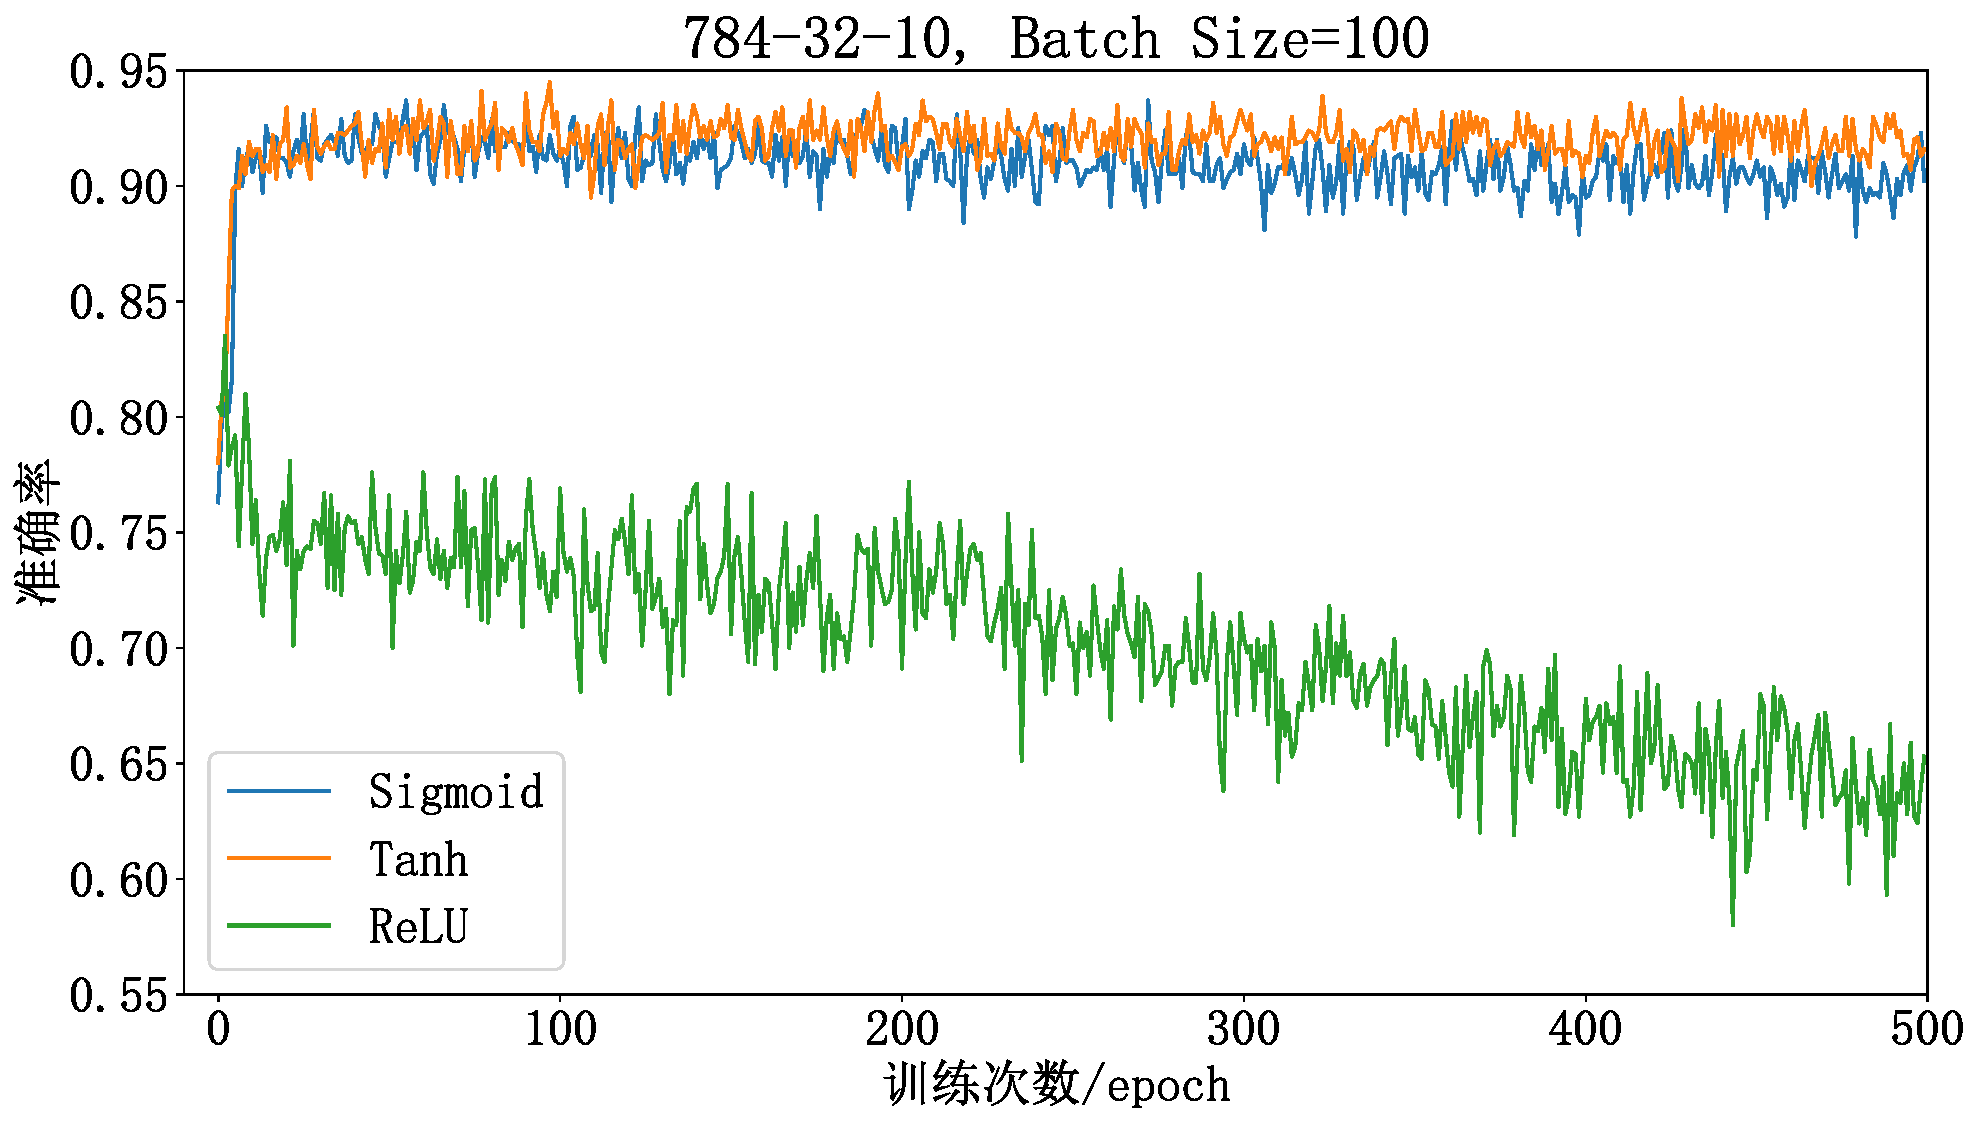
\includegraphics[scale=0.45]{diff_activation_function.pdf}
    \caption{激活函数对比}
    \label{figure-diff_activation}
\end{figure}

可以自行运行代码文件\nameref{appendix-Main}测试每次训练后前馈神经网络的准确率, 经过我们多次试验, 网络结构为783-32-10, 激活函数为Tanh, Batch Size=100, 训练$10$次左右已经可以达到$90\%$以上的准确率.

\clearpage
\begin{thebibliography}{99}  
\addcontentsline{toc}{section}{参考文献} 
\bibitem{ref-qxp}邱锡鹏. 神经网络与深度学习[M]. 北京: 机械工业出版社, 2020.3.
\bibitem{ref-prove_perceptron}Novikoff A B, 1963. On convergence proofs for perceptron[R]. DTIC Document.
\bibitem{ref-MIT}Alexander Amini, Ava Soleimany, et al. MIT Introduction to Deep Learning 6.S191, 2022 [EB/OL]. \url{http://introtodeeplearning.com/}
\bibitem{ref-ReLU}Xavier Glorot, Antoine Bordes and Yoshua Bengio. Deep sparse rectifier neural networks[C]. AISTATS. 2011.
\bibitem{ref-dropout}Srivastava N, Hinton G, Krizhevsky A, et al. Dropout: A simple way to prevent neural networks from overfitting[J]. The Journal of Machine Learning Research, 2014, 15(1): 1929-1958.
\bibitem{ref-dropout_example}Hinton G E, Srivastava N, Krizhevsky A, et al. Improving neural networks by preventing co-adaptation of feature detectors[J]. arXiv preprint arXiv:1207.0580, 2012.
\end{thebibliography}

\begin{appendices}
    \section{完整代码}
    全部代码均已上传至Github仓库\footnote{Github仓库链接: \url{https://github.com/wty-yy/Perceptron-and-FNN-by-Python}}.
    \subsection{感知器算法}\label{appendix-Perceptron}
    \pythonfile{../Python/Perceptron_main.py}
    \subsection{前馈神经网络算法}
    \paragraph{读入MNIST数据集Input.py}\label{appendix-Input}
    \pythonfile{../Python/Input.py}
    \paragraph{计时器timer.py}\label{appendix-timer}
    用于计算代码运行所用时间.
    \pythonfile{../Python/timer.py}
    \paragraph{前馈神经网络核心代码ANN.py}\label{appendix-ANN}
    \pythonfile{../Python/ANN.py}
    \paragraph{主程序Main.py}\label{appendix-Main}
    \pythonfile{../Python/Main.py}
    \clearpage
    \section{感知器迭代过程图}\label{appendix-迭代过程图}
    \begin{figure}[h]
        \centering
        \subfigure[迭代1次]
        {
            \begin{minipage}[b]{.45\linewidth}
                \centering
                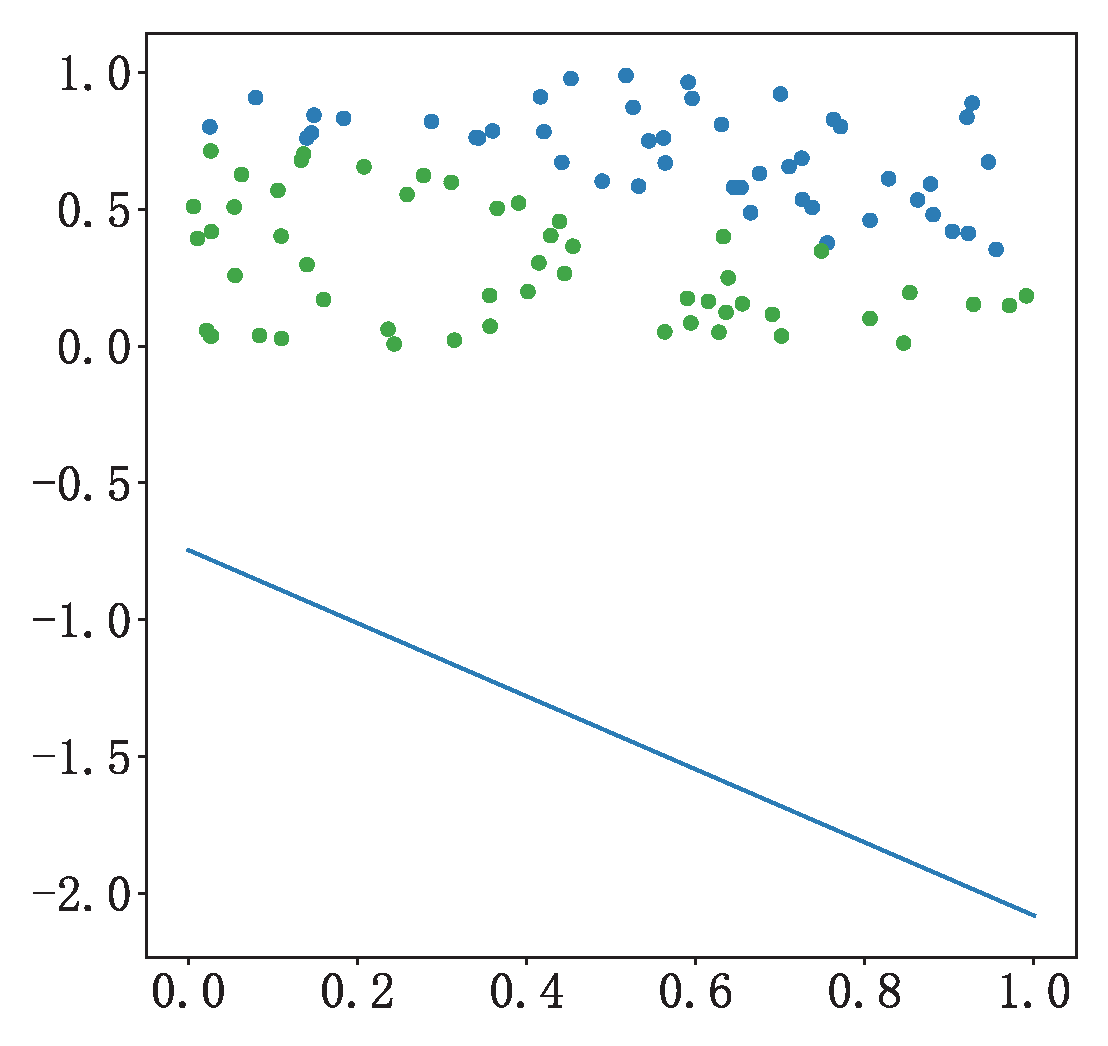
\includegraphics[scale=0.35]{1.eps}
                %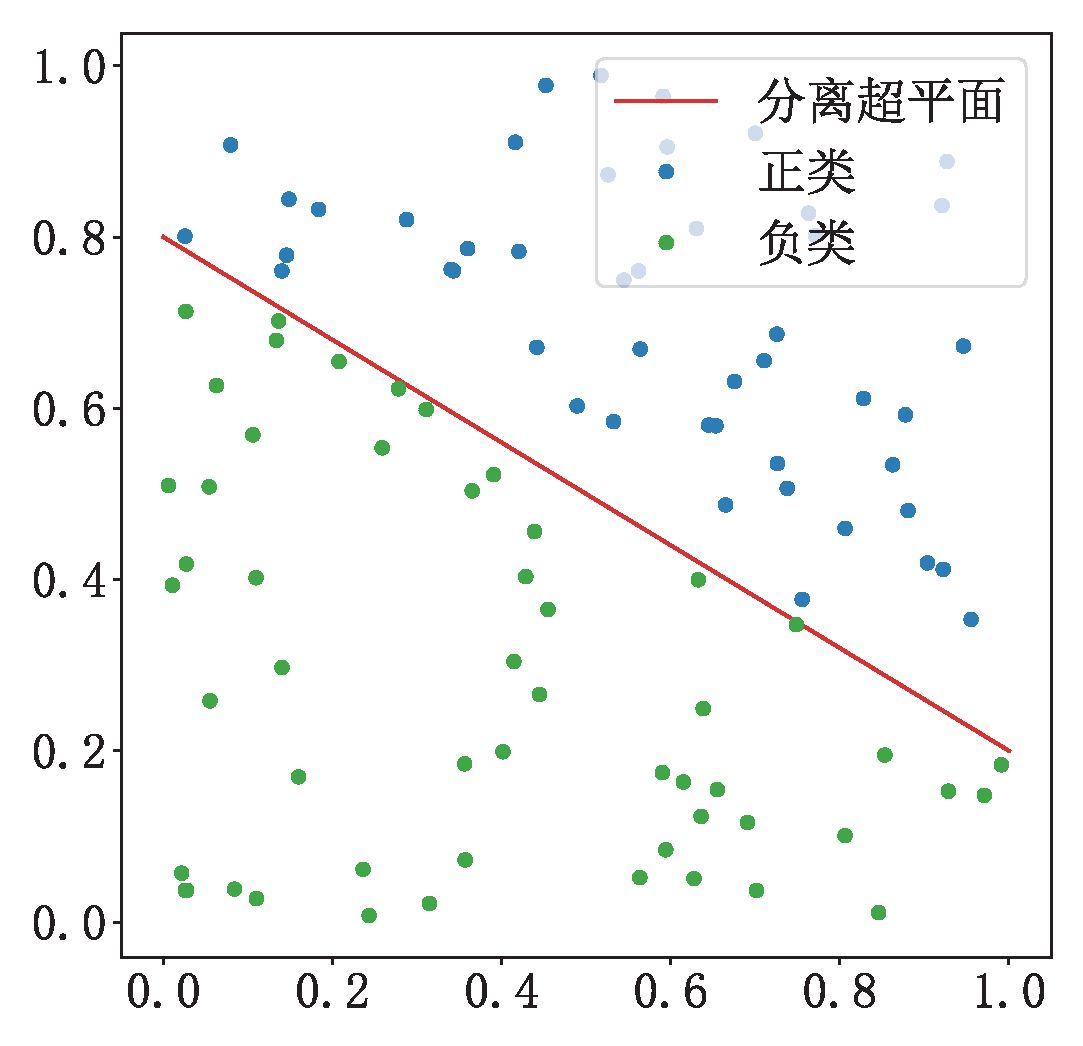
\includegraphics[width=0.8\textwidth]{分离平面.eps}
            \end{minipage}
        }
        \subfigure[迭代100次]
        {
            \begin{minipage}[b]{.45\linewidth}
                \centering
                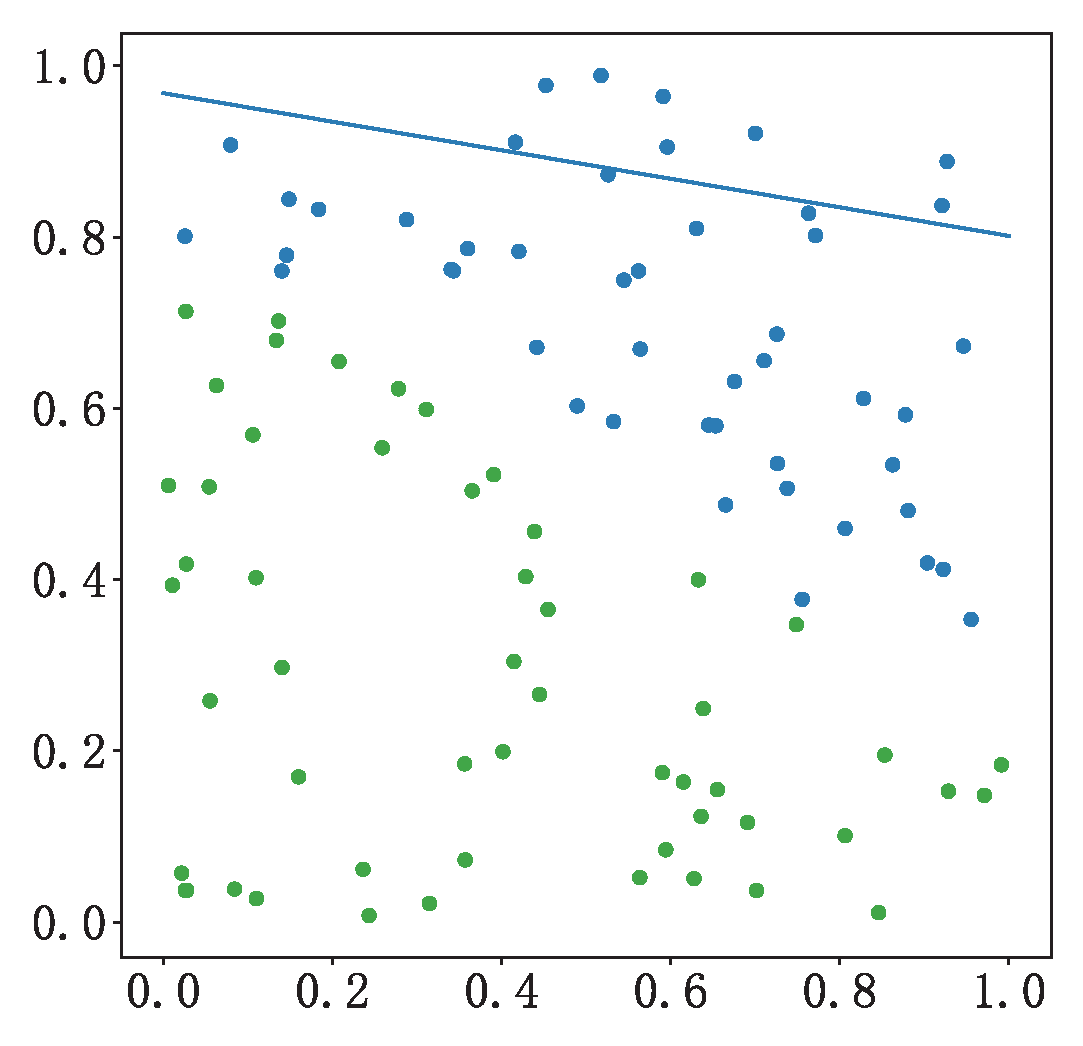
\includegraphics[scale=0.35]{100.eps}
            \end{minipage}
        }
        \subfigure[迭代500次]
        {
            \begin{minipage}[b]{.45\linewidth}
                \centering
                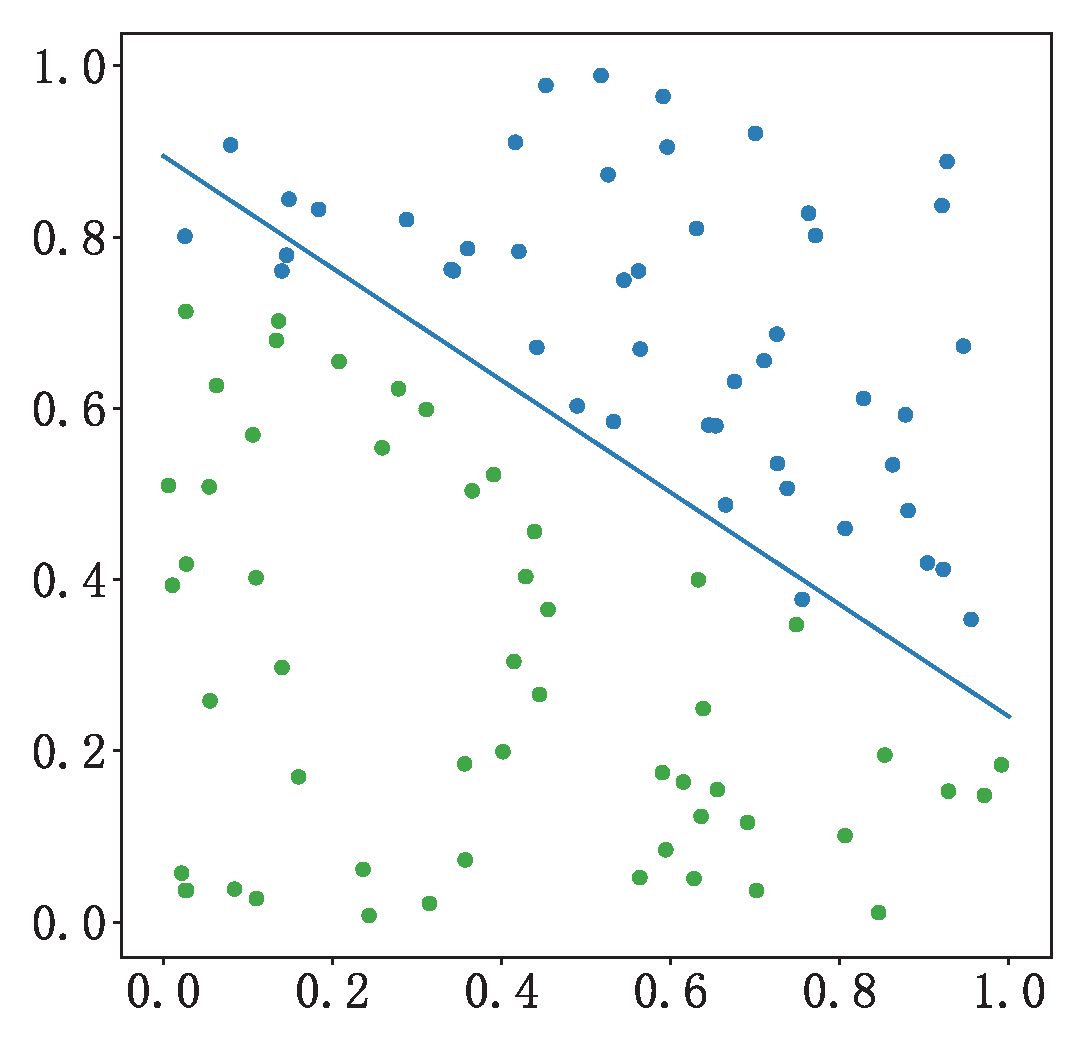
\includegraphics[scale=0.35]{500.eps}
            \end{minipage}
        }
        \subfigure[迭代2000次]
        {
            \begin{minipage}[b]{.45\linewidth}
                \centering
                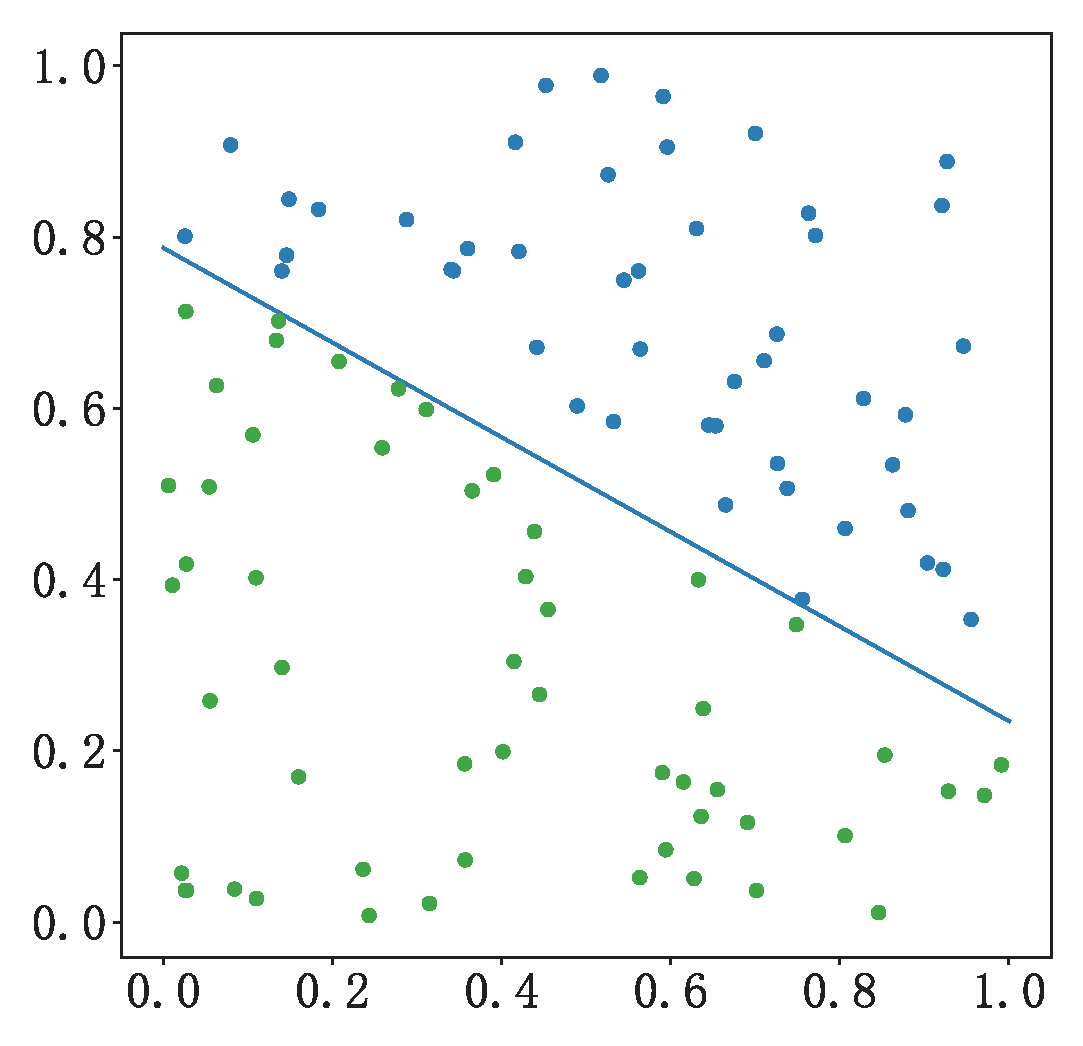
\includegraphics[scale=0.35]{2000.eps}
            \end{minipage}
        }
        \caption{迭代过程图}
        \label{figure-迭代过程图}
    \end{figure}
\end{appendices}
\end{document}

\iffalse
% 图片模板
\centerline{
    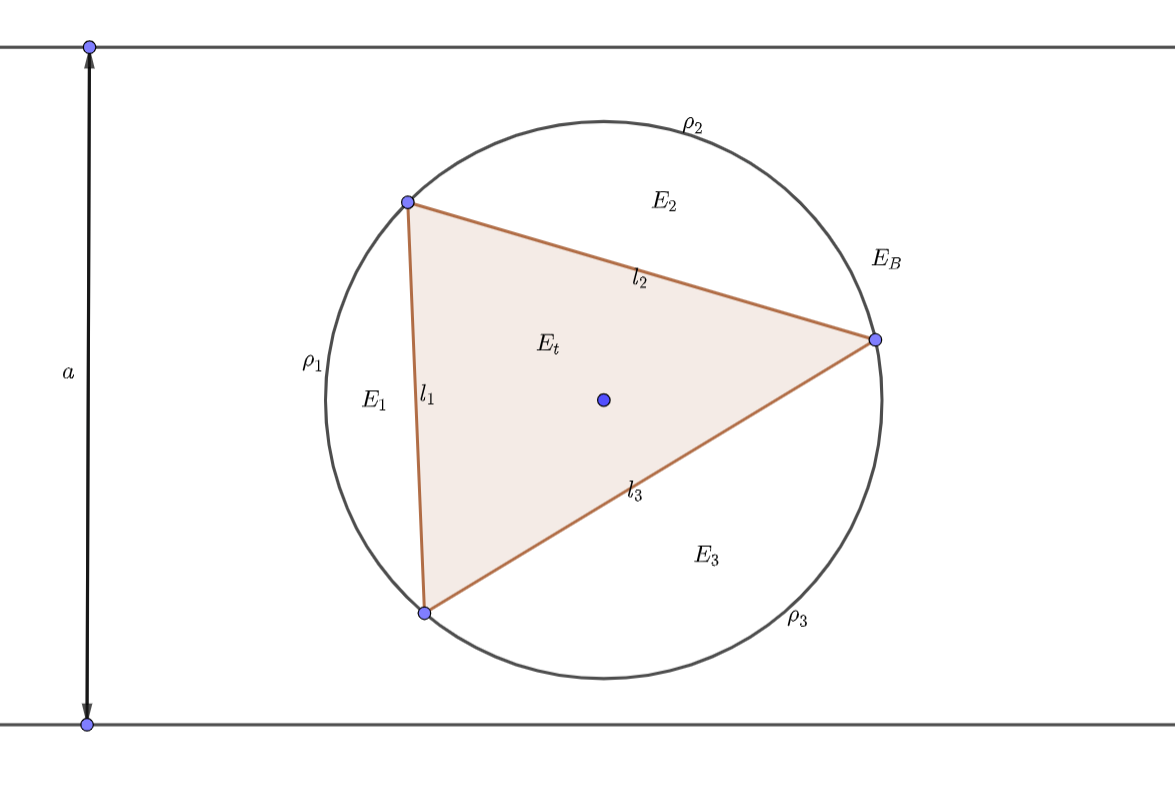
\includegraphics[width=0.8\textwidth]{figure.png}
}
\fi
\iffalse
% 表格模板
\renewcommand\arraystretch{0.8} % 设置表格高度为原来的0.8倍
\begin{table}[!htbp] % table标准
    \centering % 表格居中
    \begin{tabular}{p{1cm}<{\centering}p{1cm}<{\centering}p{3cm}<{\centering}p{5cm}<{\centering}} % 设置表格宽度
    %\begin{tabular}{cccc}
        \toprule
        $x_i$ & $f[x_1]$ & $f[x_i, x_{i+1}]$ & $f[x_i, x_{i+1}, x_{i+2}]$ \\
        \midrule
        $x_0$ & $f(x_0)$ &                  &                          \\
        $x_0$ & $f(x_0)$ & $f'(x_0)$        &                          \\
        $x_0$ & $f(x_1)$ & $\frac{f(x_1)-f(x_0)}{x_1-x_0}$ & $\frac{f(x_1)-f(x_0)}{(x_1-x_0)^2}-\frac{f'(x_0)}{x_1-x_0}$\\
        \bottomrule
    \end{tabular}
\end{table}

% 文字环绕图片, 标题加注释
\begin{wrapfigure}[13]{r}{.5\linewidth}
    \centering
    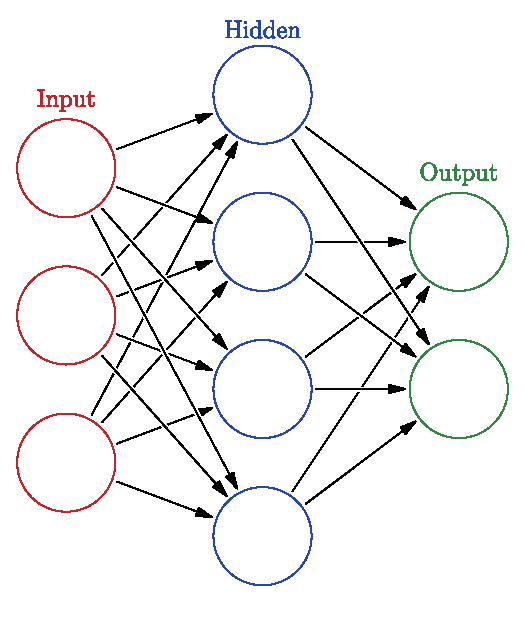
\includegraphics[scale=0.7]{neural_network.eps}
    \caption{神经网络结构\protect\footnotemark[1]}
\end{wrapfigure}
\footnotetext[1]{图片来源: \url{https://en.wikipedia.org/wiki/File:Colored_neural_network.svg}}

% 普通图片, 标题加注释
\begin{figure}[h]
    \centering
    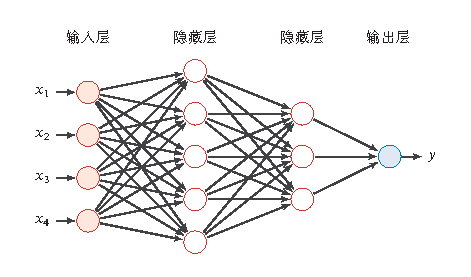
\includegraphics[scale=0.5]{前馈神经网络.eps}
    \caption{前馈神经网络\protect\footnotemark[1]}
\end{figure}
\footnotetext[1]{图片来源: 邱锡鹏, 神经网络与深度学习 \cite{ref-qxp}, 第92页}
\fi

\end{document}